\documentclass[11pt,a4paper,oneside]{book}
\usepackage{import}
\usepackage{nameref}
\usepackage[table]{xcolor}
\subimport{../}{style}
\subimport{../}{macros}
\subimport{../}{glossary}
\graphicspath{{../img/}}
\makeglossaries
\makeindex
%TODO:
% - crossref chapters & co
% - \n\n -> \n
% - soorten quotes
% - i.e. -> i.e.,
% - e.g. -> e.g.,
% - files, urls, \ldots -> \texttt


% keep in sync with title.tex title and audience
\hypersetup{
  pdftitle={VSC Cloud tutorial},
  pdfsubject={This document is a hands-on guide to the VSC cloud computing platform,
    which relies on the open-source software OpenStack.},
}

\newcommand{\osversion}{rocky}

\begin{document}

\pagestyle{empty}

 \begin{center}

\includegraphics*[width=8truecm]{logo_vsc}

\vspace*{1.5\baselineskip}

\Huge \strong{HPC Tutorial} \\
\LARGE Version 20180831.02

\ifwindows
\LARGE For Windows Users
\fi
\ifmac
\LARGE For macOS Users
\fi
\iflinux
\LARGE For Linux Users
\fi

\vspace*{.75\baselineskip}
\ifantwerpen
\includegraphics*[width=7truecm]{logo_ua}
\fi

\vspace*{0.75\baselineskip}


\normalsize\strong{Author:}

Geert Borstlap (UAntwerpen)

\vspace*{.5\baselineskip}

\strong{Co-authors:}

Kenneth Hoste, Toon Willems, Jens Timmerman (UGent)

Geert-Jan Bex (UHasselt and KU~Leuven)

Mag Selwa (KU~Leuven)

Stefan Becuwe, Franky Backeljauw, Bert Tijskens, Kurt Lust (UAntwerpen)

Bal\'azs Hajgat\'o (VUB)

\vspace*{.5\baselineskip}

Acknowledgement: VSCentrum.be

\vspace*{\baselineskip}

\begin{tabular}{ >{\centering\arraybackslash}m{0.25\textwidth}  >{\centering\arraybackslash}m{0.05\textwidth}  >{\centering\arraybackslash}m{0.20\textwidth}  >{\centering\arraybackslash}m{0.2\textwidth}} \\
\includegraphics*[width=0.2\textwidth, height=0.7in, keepaspectratio=true]{logo_auha} & \multicolumn{2}{ >{\centering\arraybackslash}m{.2\textwidth} }{\includegraphics*[width=0.2\textwidth, height=0.7in,, keepaspectratio=true]{logo_akuleuven}} & \includegraphics*[width=0.2\textwidth, height=0.7in,, keepaspectratio=true]{logo_auhl} \\
\multicolumn{2}{ >{\centering\arraybackslash}m{.32\textwidth} }{\includegraphics*[width=0.3\textwidth, height=0.7in, keepaspectratio=true]{logo_augent}} & \multicolumn{2}{ >{\centering\arraybackslash}m{.38\textwidth} }{\includegraphics*[width=0.3\textwidth, height=0.7in, keepaspectratio=false]{logo_uab}} \\
\end{tabular}
\end{center}


\cleardoublepage
\pagestyle{plain}
\strong{Audience:}

This HPC Tutorial is designed for \strong{researchers} at the
\strong{\university} and affiliated institutes who are in need of
computational power (computer resources) and wish to explore and use the High
Performance Computing (HPC) core facilities of the Flemish Supercomputing Centre (VSC)
to execute their computationally intensive tasks.


The audience may be completely unaware of the \hpc concepts but must have some
basic understanding of computers and computer programming.


\strong{\underbar{Contents:}}

This \strong{Beginners Part} of this tutorial gives answers to the typical
questions that a new \hpc user has. The aim is to learn how to make use of the
HPC.

\begin{tabular}{|p{\dimexpr 0.44\textwidth-2\tabcolsep}|>{\centering\arraybackslash}p{\dimexpr 0.12\textwidth-2\tabcolsep}|p{\dimexpr 0.44\textwidth-2\tabcolsep}|} \hline
\multicolumn{3}{|c|}{\strong{Beginners Part}} \\ \hline
\strong{Questions}                                                      & \strong{chapter} & \strong{title} \\ \hline
What is a \hpc exactly?\newline Can it solve my computational needs?    & \strong{\ref{ch:introduction-to-hpc}} & \nameref{ch:introduction-to-hpc} \\ \hline
How to get an account?                                                  & \strong{\ref{ch:getting-a-hpc-account}} & \nameref{ch:getting-a-hpc-account} \\ \hline
How do I connect to the \hpc and transfer my files and programs?        & \strong{\ref{ch:preparing-the-environment}} & \nameref{ch:preparing-the-environment} \\ \hline
How to start background jobs?                                           & \strong{\ref{ch:running-batch-jobs}} & \nameref{ch:running-batch-jobs} \\ \hline
How to start jobs with user interaction?                                & \strong{\ref{ch:running-interactive-jobs}} & \nameref{ch:running-interactive-jobs} \\ \hline
Where do the input and output go? Where to collect my results?          & \strong{\ref{ch:running-jobs-with-input-output-data}} & \nameref{ch:running-jobs-with-input-output-data} \\ \hline
Can I speed up my program by exploring parallel programming techniques? & \strong{\ref{ch:multi-core-jobs-parallel-computing}} & \nameref{ch:multi-core-jobs-parallel-computing} \\ \hline
Can I start many jobs at once?                                          & \strong{\ref{ch:multi-job-submission}} & \nameref{ch:multi-job-submission} \\ \hline
What are the rules and priorities of jobs?                              & \strong{\ref{ch:hpc-policies}} & \nameref{ch:hpc-policies} \\ \hline
\end{tabular}

The \strong{Advanced Part} focuses on in-depth issues. The aim is to assist the
end-users in running their own software on the \hpc.

\begin{tabular}{|p{\dimexpr 0.44\textwidth-2\tabcolsep}|>{\centering\arraybackslash}p{\dimexpr 0.12\textwidth-2\tabcolsep}|p{\dimexpr 0.44\textwidth-2\tabcolsep}|} \hline
\multicolumn{3}{|c|}{\strong{Advanced Part}} \\ \hline
\strong{Questions}                           & \strong{chapter} & \strong{title} \\ \hline
Can I compile my software on the \hpc?       & \strong{\ref{ch:compiling-and-testing-your-software-on-the-hpc}}      & \nameref{ch:compiling-and-testing-your-software-on-the-hpc} \\ \hline
What are the optimal Job Specifications?     & \strong{\ref{ch:fine-tuning-job-specifications}}      & \nameref{ch:fine-tuning-job-specifications} \\ \hline
%How do I check my programs at runtime?       & \strong{\ref{ch:monitoring-cluster-utilization}}      & \nameref{ch:monitoring-cluster-utilization} \\ \hline
%Can I stop my program and continue later on? & \strong{\ref{ch:checkpointing}}      & Checkpointing \\ \hline
Do you have more examples for me?            & \strong{\ref{ch:program-examples}}      & \nameref{ch:program-examples} \\ \hline
Any more advice?                             & \strong{\ref{ch:best-practices}}      & \nameref{ch:best-practices} \\ \hline
\end{tabular}

The \strong{Annexes} contains some useful reference guides.

\begin{tabular}{|l|c|} \hline
\multicolumn{2}{|c|}{\strong{Annex}} \\ \hline
\strong{Title}             & \strong{chapter} \\ \hline
\nameref{ch:quick-reference-guide} & \strong{\ref{ch:quick-reference-guide}} \\ \hline
\nameref{ch:torque-options}& \strong{\ref{ch:torque-options}} \\ \hline
\nameref{ch:useful-linux-commands}& \strong{\ref{ch:useful-linux-commands}} \\ \hline
\end{tabular}


\strong{\underbar{Notification:}}

In this tutorial specific commands are separated from the accompanying text:

\begin{prompt}
%\shellcmd{commands}%
\end{prompt}

These should be entered by the reader at a command line in a Terminal on the \hpcInfra. They appear in all exercises preceded by a \$ and printed in \textbf{bold}. You'll find those actions in a grey frame.

\keys{Button} are menus, buttons or drop down boxes to be pressed or selected.

``Directory'' is the notation for directories (called ``folders'' in
Windows terminology) or specific files. (e.g., ``\homedir'')

``Text'' Is the notation for text to be entered.

\begin{tip}
A ``Tip'' paragraph is used for remarks or tips.
\end{tip}

\strong{\underbar{More support:}}

Before starting the course, the example programs and configuration files used in this Tutorial must be copied to your home directory, so that you can work with your personal copy. If you have received a new VSC-account, all examples are present in an ``\examplesdir'' directory.

\begin{prompt}
%\shellcmd{cp --r \examplesdir \tilde/}%
%\shellcmd{cd}%
%\shellcmd{ls}%
\end{prompt}

They can also be downloaded from the VSC website at
\url{https://www.vscentrum.be}.
Apart from this \hpc Tutorial, the documentation on the VSC website
will serve as a reference for all the
operations.


\begin{tip}
The users are advised to get self-organised. There are
only limited resources available at the \hpc, which are best effort based.
The \hpc cannot give support for code fixing, the user applications and own
developed software remain solely the responsibility of the end-user.
\end{tip}

More documentation can be found at:

\begin{enumerate}
  \item  VSC documentation: \url{https://www.vscentrum.be/en/user-portal}
  \ifantwerpen
    \item CalcUA Core Facility web pages: \url{https://www.uantwerpen.be/hpc}
  \fi
  \ifbrussel
    \item \hpcname documentation: \url{http://cc.ulb.ac.be/hpc}
  \fi
  \ifgent
    \item \hpcname documentation: \url{http://hpc.ugent.be/userwiki}
  \fi
  \item  External documentation (TORQUE, Moab): \url{http://docs.adaptivecomputing.com}
\end{enumerate}

This tutorial is intended for users who want to connect and work on the HPC of the \strong{\university}.

This tutorial is available in a Windows, Mac or Linux version.

This tutorial is available for UAntwerpen, UGent, KU~Leuven, UHasselt and VUB users.

Request your appropriate version at \hpcinfo.

\strong{\underbar{Contact Information:}}

We welcome your feedback, comments and suggestions for improving the \hpc
Tutorial  (contact: \hpcinfo).

For all technical questions, please contact the \hpc staff:

\inputsite{contact-information}




\glsdisablehyper
\glstoctrue
\printglossaries

\cleardoublepage
%\addcontentsline{toc}{chapter}{Index}
\printindex


\tableofcontents

\pagestyle{fancy}
\chapter*{Introduction}
The VSC cloud platform uses the open-source software
\href{https://openstack.org}{\gls{OpenStack}}, version ``\osversion''.
This guide explains the specifics of the VSC environment, and provides
a hands-on introduction to OpenStack.  For reference, you should
consult the OpenStack project's own documentation at
\url{https://docs.openstack.org}.

%%% Local Variables:
%%% mode: latex
%%% TeX-master: "intro-Cloud"
%%% End:


\chapter{Access to the VSC Cloud}
Access to the VSC Cloud is linked to the central VSC account system
(\href{https://account.vscentrum.be}{account.vscentrum.be}), so you do
not need a separate login or password.  In order to use the cloud
services,
\begin{itemize}
\item you need an active VSC account and
\item your account must be a member of one or more OpenStack projects.
\end{itemize}
New users can obtain an account at
\href{https://www.vscentrum.be/cluster-doc/account-request}{www.vscentrum.be/cluster-doc/account-request}.
Contact \cloudinfo if you want to start a new OpenStack project, or
join an existing one.

You can interact with the VSC Cloud using the OpenStack Dashboard, a
web interface, or the OpenStack command line interface, which you can
use from any system, and which is installed for you on the UGent login
node \lstinline{login.hpc.ugent.be}.  You can log in to the Dashboard
using the VSC accountpage, as illustrated in the next section.  To get
access from the command line interface, you'll need to obtain an
application credential, as explained in section \ref{sec:appl-cred}.

These restrictions do not apply to someone who simply wishes to access
an existing VM running in the cloud.  VSC Cloud projects can decide
themselves who gets access to their VM's, and how.

\section{Dashboard Login}\label{sec:dashboard-login}
You can access the OpenStack web interface, or Dashboard, via \href{https://cloud.vscentrum.be}{cloud.vscentrum.be}.

To log in, choose the (default) authentication method \emph{VSC Accountpage} and click \strong{Connect}.
\begin{center}

\includegraphics[width=0.5\textwidth]{img/cloud_login_1.png}
\end{center}

From here on, follow the standard procedure to log in to your VSC
account, using your home institution's single sign-on system.  You can
find a detailed description in the HPC tutorial at
\href{https://www.vscentrum.be/support/tut-book/vsc-tutorials}{www.vscentrum.be/support/tut-book/vsc-tutorials}.
The following chapters explain how to accomplish basic tasks using the Dashboard.

\section{Application Credentials}\label{sec:appl-cred}
If you want to use the OpenStack command line interface  --- or, for advanced users, use the OpenStack APIs directly --- you need to identify yourself using an application credential.  An application credential contains a secret piece of information which grants access to an OpenStack project on your behalf.

You can create an application credential using the dashboard:
\begin{enumerate}
\item Log in to the dashboard, and, if you are a member of more than
  one project, select the project for which you want to create an
  application credential.
\item Open the \textbf{Identity} tab, and click \textbf{Application
    Credentials}.
\item You can now see an overview of your application credentials
  (initially none).  Click \textbf{Create Application Credential}.
\item Fill out the \textbf{Create Application Credential} dialog:
  \begin{description}
  \item[Name, Description] Choose a name (mandatory) and description
    that remind you of the purpose of this credential.
  \item[Secret] We recommend to leave this empty, in which case
    OpenStack will generate a random secret for you.
  \item[Expiration Date, Expiration Time] It is good practice make the
    token expire.  An expiration date limits the impact if the secret
    is accidentally exposed, and you can always create a new
    credential when an old one is expired.
  \item[Roles] A role defines a set of access rights. By selecting a
    subset of roles for this credential, you can limit the access
    rights granted by this credential.  It is a good idea to select
    only the minimal set of roles required for the task you want to
    accomplish.
  \end{description}
  Click \textbf{Create Application Credential}.
\item A summary dialog with the credential's id, name, and secret is
  displayed.  If you close the window, you can't retrieve the secret
  anymore, so you should save it now.  A convenient solution is to
  download the openrc file, a shell script that sets the appropriate
  environment variables for the command line interface.
\end{enumerate}

The newly created credential is now shown in the overview.  If you
accidentally expose a credential somewhere, you should delete it here
to prevent unauthorized access to the system.

%%% Local Variables:
%%% mode: latex
%%% TeX-master: "intro-Cloud"
%%% End:


\chapter{The OpenStack Dashboard}
This chapter briefly describes the different components of
\gls{Horizon}, the \gls{OpenStack Dashboard}.  You can read the
official documentation at
\url{https://docs.openstack.org/horizon/\osversion/user}.
\strong{Note:} the following features are not available for VSC cloud
users, and have been removed from the dashboard:
\begin{itemize}
\item Consistency Group Snapshots (``Volumes'' tab);
\item Managing your own networks and routers (``Network'' tab);
\item Sharing networks (``Share'' tab).
\end{itemize}
Please contact \cloudinfo if you need access to one of these disabled
features.

After login the user will be navigated to the Overview tab of the dashboard.
\begin{center}
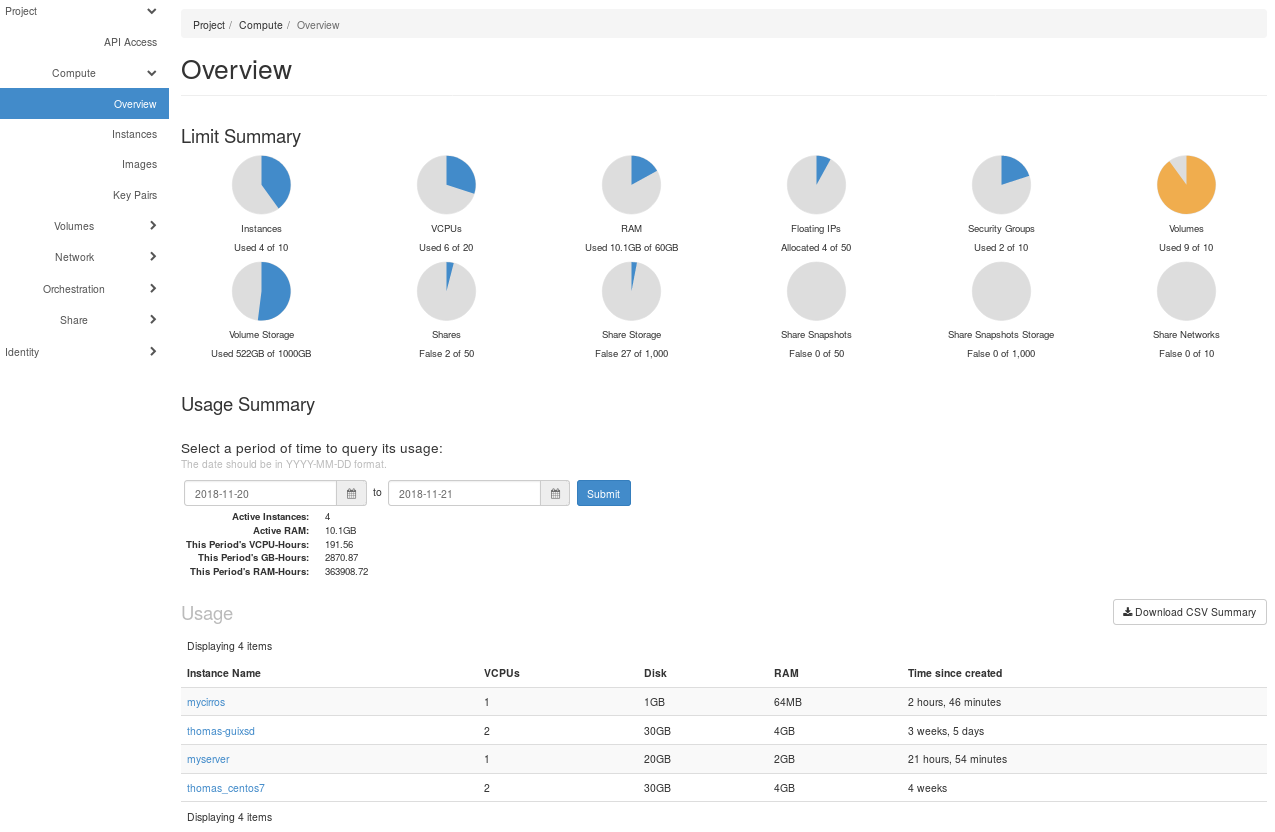
\includegraphics[scale=0.3]{img/tab-compute-overview.png}
\end{center}

\section*{OpenStack dashboard - Project
  tab}\label{openstack-dashboard---project-tab}
Resources (instances, data volumes, networks, \ldots) in OpenStack are
organized into different projects, and every user is a member of one
or more projects.  Every project member has full access to all of the
project's resources.

From the Project tab, you can access the following categories:
\begin{itemize}
\item
  API Access: View API endpoints.
\end{itemize}

\subsection*{\texorpdfstring{Compute
tab}{Compute tab}}\label{compute-tab}

\begin{itemize}
\item
  Overview: View reports for the project.
\item
  Instances: View, launch, create a snapshot from, stop, pause, or
  reboot instances, or connect to them through VNC.
\item
  Images: View images and instance snapshots created by project users,
  plus any images that are publicly available. Create, edit, and delete
  images, and launch instances from images and snapshots.
\item
  Key Pairs: View, create, edit, import, and delete key pairs.
\item
  Server Groups: Server groups provide a mechanism to group servers according to certain policy.
\end{itemize}

\subsection*{\texorpdfstring{Volumes
tab}{Volumes tab}}\label{volumes-tab}

\begin{itemize}
\item
  Volumes: View, create, edit, and delete volumes.
\item
  Snapshots: View, create, edit, and delete volume snapshots.
\end{itemize}

\subsection*{\texorpdfstring{Network
tab}{Network tab}}\label{network-tab}

\begin{itemize}
\item
  Network Topology: View the network topology.
\item
  Networks: Create and manage public and private networks.
\item
  Security Groups: View, create, edit, and delete security groups and
  security group rules..
\item
  Floating IPs: Allocate an IP address to or release it from a project
\end{itemize}

\subsection*{\texorpdfstring{Orchestration
tab}{Orchestration tab}}\label{orchestration-tab}

\begin{itemize}
\item
  Stacks: Use the REST API to orchestrate multiple composite cloud applications.
\item
  Resource types: Show a list of all the supported resource types for HOT templates.
\item
  Template versions: The version of a Heat template specifies the format of the template and also the corresponding features that will be validated and supported.
\item
  Template generator: Provides the user with the option to build and edit templates. 
\end{itemize}

\subsection*{\texorpdfstring{Share
tab}{Shares tab}}\label{shares-tab}

\begin{itemize}
\item
  Shares: A share is a remote, mountable file system. Users can mount a share to and access a share from several hosts by several users at a time.
\end{itemize}

\section*{OpenStack dashboard - Identity
tab}\label{openstack-dashboard---identity-tab}

From the Identity tab, you can access the following categories:

\begin{itemize}
\item
  Projects: View, create, assign users to, remove users from, and delete
  projects.
\item
  Users: View, create, enable, disable, and delete users.
\item
  Application Credentials: With application credentials, a user can grant their applications limited access to their cloud resources.
\end{itemize}

%%% Local Variables:
%%% mode: latex
%%% TeX-master: "intro-OpenStack"
%%% End:


\chapter{Upload and manage images}\label{cha:upload-manage-images}

A virtual machine image, referred to in this document simply as an
image, is a single file that contains a virtual disk that has a
bootable operating system installed on it. Images are used to create
virtual machine instances within the cloud.  The image files
themselves are never modified, but you can copy the image into a persistent instance (see chapter \ref{cha:launch-manage-inst}).

As a user of the VSC cloud, you can upload and manage your own virtual
machine images.  For information about creating image files, see the
\href{https://docs.openstack.org/image-guide/}{\emph{OpenStack Virtual
    Machine Image Guide}}.

\strong{Note:} Shared storage in the VSC cloud is connected to a separate network, which is only accessible from within the OpenStack environment.  Therefore, if you want to access your VM from outside of OpenStack, and use the shared storage at the same time, you must make sure your VM image is configured use multiple network interface cards (NICs).

You can choose who can access an image you have created.  The following access policies for images exist:
\begin{description}
\item[public] Public images are provided by the VSC, and can be accessed by all users.
\item[private] If you create a private image, only members of the same
  project have access.
\item[shared] You can also choose to share your image with a list of
  other projects.
\item[community] Community images are user-created images which are
  freely accessible to all other users.
\end{description}

\strong{Note:} You can also use the \textbf{openstack} and
\textbf{glance} command-line clients or the Image service to manage
images.

\subsubsection{Upload an image}
Follow this procedure to upload an image to a project:

\begin{enumerate}
\item Open the Compute tab and click Images category.
\item Click Create Image.

  The Create An Image dialog box appears.
  \begin{center}
    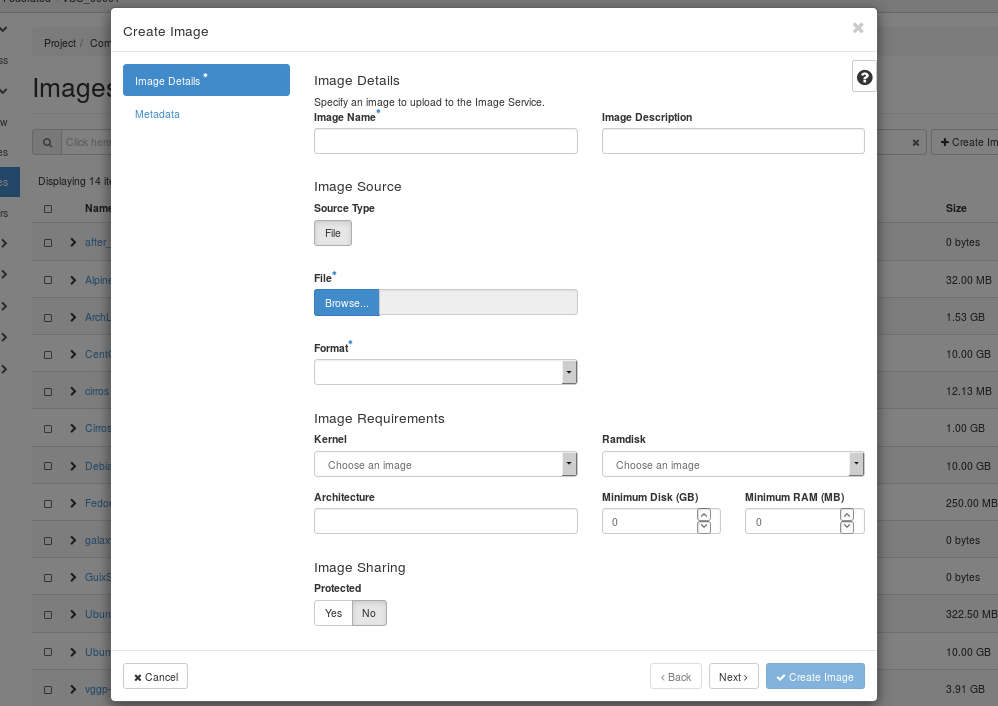
\includegraphics[scale=0.4]{img/tab-compute-images-create.png}
  \end{center}

\item Enter the following values:
  \begin{description}
  \item[Image Name] Enter a name for the image.
  \item[Image Description] Enter a brief description of the image.
  \item[Image Source] Choose the image source from the dropdown list. Your
    choices are Image Location and Image File.
  \item[Image File or Image Location] Based on your selection for
    Image Source, you either enter the location URL of the image in
    the Image Location field, or browse for the image file on your
    file system and add it.
  \item[Format] Select the image format (for example, QCOW2) for the
    image.
  \item[Architecture] Specify the architecture. For example,
    \strong{i386} for a 32-bit architecture or \strong{x86\_64} for a
    64-bit architecture.
  \item[Minimum Disk (GB)] Leave this field empty.
  \item[Minimum RAM (MB)] Leave this field empty.
  \item[Copy Data] Specify this option to copy image data to the Image
    service.
  \item[Visibility] The access permission for the
    image. \strong{Public} or \strong{Private}.
  \item[Protected] Select this check box to ensure that only users
    with permissions can delete the image. \strong{Yes} or
    \strong{No}.
  \item[Image Metadata] Specify this option to add resource
    metadata. The glance Metadata Catalog provides a list of metadata
    image definitions.  (\strong{Note:} Not all cloud providers enable
    this feature.)
  \end{description}
\item Click \strong{Create Image}.

  The image is queued to be uploaded. It might take some time before
  the status changes from Queued to Active.
\end{enumerate}

Another way to create an image is to check-mark on the left side one of the available images and then click on Launch on the right of the screen. That way the mandatory fields in 'Image Details' tab in the 'Create Image' pop-up dialog are automatically filled and the user will be directly presented with the 'Launch Instance'.

\begin{center}
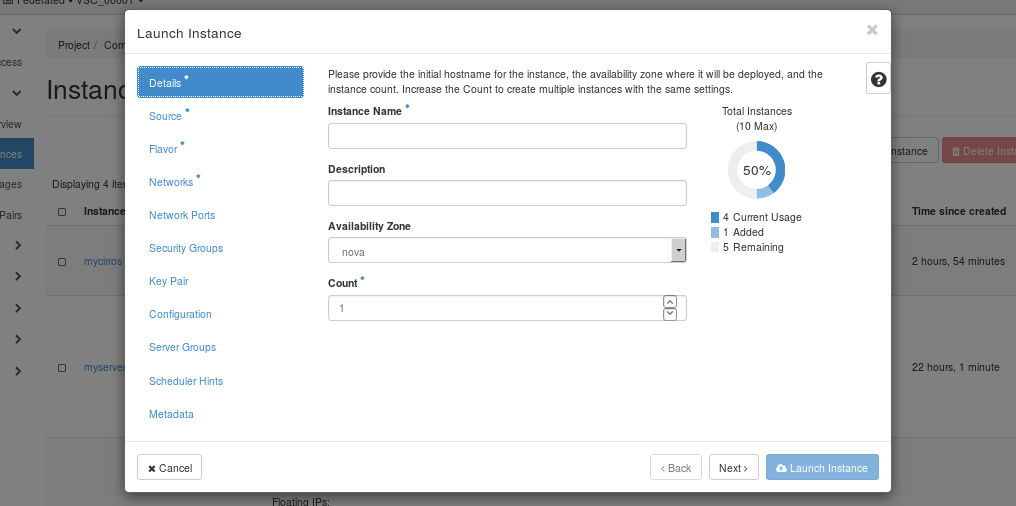
\includegraphics[scale=0.5]{img/tab-compute-instances-launch.png}
\end{center}

\subsubsection{Update an image}

Follow this procedure to update an existing image.

\begin{enumerate}
\item    Log in to the dashboard.
\item Select the appropriate project from the drop down menu at the
  top left.
\item    Select the image that you want to edit.
\item In the Actions column, click the menu button and then select
  Edit Image from the list.
\item In the Edit Image dialog box, you can perform various
  actions. For example:
  \begin{itemize}
  \item    Change the name of the image.
  \item    Change the description of the image.
  \item    Change the format of the image.
  \item    Change the minimum disk of the image.
  \item    Change the minimum RAM of the image.
  \item    Select the Public button to make the image public.
  \item    Clear the Private button to make the image private.
  \item    Change the metadata of the image.
  \end{itemize}
\item  Click Edit Image.
\end{enumerate}

%%% Local Variables:
%%% mode: latex
%%% TeX-master: "intro-Cloud"
%%% End:


\chapter{Instance types and flavors}

VSC Tier1 Cloud provides several virtual machine instance types
and flavors to fit different use cases.
Each instance type provides several flavor sizes to give different
combinations of CPU, memory, GPU and network resource.

\section{Instance Types}\label{sec:instance-types}
The following table provides the current main instance types available
from VSC Tier1 Cloud infrastructure:

\begin{table}[h!]
\centering
\begin{tabular}{ |p{6cm}|p{4cm}|p{5cm}| }
  \hline
  \rowcolor{lightgray} \textbf{UPSv1} & \textbf{CPUv1} & \textbf{GPUv1} \\
  \hline
  \begin{itemize}
    \item AMD Epyc 7542 2.9GHz
    \item vCPU oversubscription 2:1
    \item 25Gbit Ethernet
    \item Uninterruptible Power Supply (UPS)
  \end{itemize}
  &
  \begin{itemize}
    \item Intel Xeon CPU E5-2670 2.60GHz
    \item 10Gbit Ethernet
  \end{itemize}
  &
  \begin{itemize}
    \item AMD Epyc 7542 2.9GHz
    \item 25Gbit Ethernet
    \item NVIDIA Tesla 4 GPU
  \end{itemize}
  \\
  \hline
\end{tabular}
\caption{Instance types hardware profiles}
\label{table:instance-type}
\end{table}

Each instance type is appropriate for different workloads. From regular 
CPU usage (\strong{CPUv}\emph{<version>} instance types), to high performance 
GPU computations (\strong{GPUv}\emph{<version>}) or VMs connected to 
uninterruptible power supplies (\strong{UPSv}\emph{<version>}). VMs using UPS 
flavor types will be keep up and running even if the data centre suffers
an unexpected power cut.

VSC Tier-1 Cloud instance types also provide different kind of network
performance specifications. All the instance types are able to connect
to the available networks: public network, VSC network and shared filesystem
network (NFS). VSC and shared file system networks are only available
by project's request.

VSC network gives an optimal path towards other VSC sites (ideal for high
perfomance connections between different clusters and services within VSC).

\strong{Note:} Cloud projects should request VSC network if they want to
connect to VSC Data component (\url{https://www.vscentrum.be/data}) with iRODS
and Globus from their Tier1 Cloud VMs.

On the other hand, the shared filesystem network is required by the OpenStack
shared filesystem service (Manila) (see chapter \ref{cha:shared-file-systems}
for more information).


\section{Flavor Sizes}\label{sec:flavor-sizes}
A flavor size is a set of virtualized hardware resouces to a virtual
machine (VM) instance like system memory size, virtual CPU (vCPU)
or the root filesystem size. 

The flavor's root size is the amount of disk space
used by the root (\emph{/}) partition, an ephemeral disk that the
base image is copied into (see section \ref{launch-an-instance} for
more information about VM persistent/non-persistent instances).

The flavor's root ephemeral storage is only used when booting from
a non-persistent VM but not from a persistent storage volume or
persistent VM.
The flavor's root ephemeral size is not taken into account to
calculate the project's local storage quota either. You can also
create a persistent volume and choose the desired filesystem size for
your persistent VM during the instantiation.
VM persistent volumes could be resized later if that is necessary
(see next chapter \ref{cha:launch-manage-inst} for more information).

VSC Tier-1 Cloud VM flavors are grouped by instance types
(see table \ref{table:instance-type}). The current flavor sizes are
available for each instance type and can be used in different
combinations to fit different workload hardware requirements.

\begin{table}[h!]
\centering
\begin{tabular}{ |p{3cm}|p{3cm}|p{3cm}|p{3cm}| }
  \hline
  \rowcolor{lightgray} \textbf{Flavor Size} & \textbf{RAM} & \textbf{Root Disk} & \textbf{vCPUs} \\
  \hline
  small & 2Gb & 20Gb & 1 \\
  \hline
  medium & 4Gb & 30Gb & 2 \\
  \hline
  large & 8Gb & 40Gb & 4 \\
  \hline
  xlarge & 16Gb & 40Gb & 8 \\
  \hline
  1\_2xlarge & 62Gb & 40Gb & 8 \\
  \hline
  2xlarge & 62Gb & 40Gb & 16 \\
  \hline
  3xlarge & 120Gb & 80Gb & 16 \\
  \hline
\end{tabular}
\caption{Flavor sizes}
\label{table:flavor-size}
\end{table}

E.g. \strong{GPUv1}.\emph{large} OpenStack flavor will instantiate a
VM with 4 AMD Epyc 7542 2.9GHz CPUs, with a NVIDIA Tesla 4 GPU, 8GB
of ram, 40Gb of root disk and connected to the UPS.

%%% Local Variables:
%%% mode: latex
%%% TeX-master: "intro-Cloud"
%%% End:


\chapter{Configure access and security for instances}\label{cha:conf-access-secur}
The security and accessibility of your cloud resources is governed by
a few different aspects, which we discuss more detail in the following
sections:
\begin{itemize}
\item Each cloud project can use one floating IP, a public IP address
  which you'll need to connect to the resources you want to access.
\item By default, the UGent firewall blocks most IP addresses and
  ports.  Only the port range 50000-60000 for the floating IP
  addresses is open by default.  Contact \cloudinfo if you need to
  access other ports from the outside world.
\item Instances must connect to the project's \_vm network in order to
  communicate.
\item The OpenStack environment has its own internal firewalls, which
  block most ports of your instances.  If you want to access specific
  ports of your instances, you must create ``Security Groups'' which
  allow access to those ports.
\item If you want to access your instances using SSH key
  authentication, you need to make sure the appropriate keys are
  installed on the those instances.  OpenStack has some support for
  the automatic inclusion of SSH keys for instance administrators.
  For your convenience, public keys you have added to your VSC account
  are automatically available in OpenStack.
\end{itemize}
For other access methods, or SSH authentication for a wider set of
users, you'll need to set up some form of identity management
yourself.  This system administration task is beyond the scope of our
tutorial.

\section{Security Groups}\label{sec:security-groups}
OpenStack security groups are sets of IP filter rules that define
networking access.  You can then assign one or more security groups to
your instances.

In the VSC cloud, each project contains a default security group,
which allows you to ping instances and connect using SSH on the
default port 22.  If you want to access other ports on your instances,
create new security groups with the appropriate rules and assign them
to the instances.

\section{SSH key pairs}\label{sec:ssh-key-pairs}
When an instance is launched, OpenStack can automatically install a
public SSH key on it, so as to give anyone with the corresponding
private key admin access.  For this ``key pair injection\footnote{The
  OpenStack documentation and interfaces consistently refer to ``SSH
  pairs'', but of course only the public key of each pair is stored in
  the OpenStack environment, while the private key should be kept
  secure by the owner.}'' to work, the image that the instance is
based on must contain the \textbf{cloud-init} package, or have in
place another mechanism in place that will interact with the OpenStack
metadata server to install the appropriate key.  For general
instructions on SSH keys, we refer to chapter 2 of
\href{https://www.vscentrum.be/support/tut-book/vsc-tutorials}{the VSC
  HPC tutorial}.

If you have generated a key pair with an external tool, you can import
it into OpenStack. The key pair can be used for multiple instances
that belong to a project. For more information, see section
\ref{import-a-key-pair}.

\strong{Note:} The public keys from your VSC account are automatically
available in your VSC Cloud projects, so you can immediately inject
one of your existing into your instances.  Of course, you can also
import new keys into OpenStack, which are not coupled to your VSC
account.  If you want to give other parties SSH access to VM's, you
must manage the keys using some other method.  \strong{Never} upload
SSH keys for other users to your VSC account.

\strong{Note:} Every OpenStack user account has its own collection of
SSH keys for every project.  To share a public key between multiple
users of the same project, each user needs to import it in the
OpenStack project.

\subsection*{Add a key pair}\label{add-a-key-pair}
\begin{enumerate}
\item Open the Compute tab.
\item Click the Key Pairs tab, which shows the key pairs that are
  available for this project.
\item Click Create Key Pair.
\item In the Create Key Pair dialog box, enter a name for your key
  pair, and click Create Key Pair.
\item Respond to the prompt to download the key pair.
\item Save the \textbf{*.pem} file locally.
\item To change its permissions so that only you can read and write to
  the file, run the following command:

  \begin{prompt}
      %\shellcmd{chmod 0600 yourPrivateKey.pem}
  \end{prompt}

  \strong{Note:} If you are using the \gls{OpenStack Dashboard} from a
  Windows computer, use PuTTYgen to load the \textbf{*.pem} file and
  convert and save it as \textbf{*.ppk}.  For more information see the
  \href{https://winscp.net/eng/docs/ui_puttygen}{\emph{WinSCP web page
      for PuTTYgen}}, and chapter 2 of
  \href{https://www.vscentrum.be/support/tut-book/vsc-tutorials}{the
    VSC HPC tutorial}.

\item To make the key pair known to SSH, run the \textbf{ssh-add}
  command.

  \begin{prompt}
    %\shellcmd{ssh-add yourPrivateKey.pem}
  \end{prompt}
\end{enumerate}

\subsection*{Import a key pair}\label{import-a-key-pair}
\begin{enumerate}
\item Open the Compute tab.
\item Click the Key Pairs tab, which shows the key pairs that are
  available for this project.
\item Click Import Key Pair.
\item In the Import Key Pair dialog box, enter the name of your key
  pair, copy the public key into the Public Key box, and then click
  Import Key Pair.
\end{enumerate}

The Compute database registers the public key of the key pair.

The \gls{OpenStack Dashboard} lists the key pair on the Key Pairs tab.

\section{The \_vm and \_nfs networks}\label{sec:_vm-_nfs-networks}
Each project in the VSC cloud has its own network
\texttt{\emph{<projectname>}\_vm} and --- if the project uses shares ---
\texttt{\emph{<projectname>}\_nfs}.

Instances should use the \_vm network for communication.  When an
instance is created in \gls{OpenStack} and connected to the \_vm
network, it is automatically assigned a fixed IP address in that
network. This IP address is permanently associated with the instance
until the instance is terminated.  However, the \_vm network can only
be reached from within the OpenStack environment.

\section{Floating IP addresses}\label{sec:floating-ip}
The \_vm and \_nfs networks can only be reached from within the
OpenStack environment.  If you need to access an instance from the
outside, you need to use one of your project's floating IP addresses,
which are public IP adresses.  Unlike fixed IP addresses, floating IP
addresses can have their associations modified at any time, regardless
of the state of the instances involved.

This section explains how to make your instance accessible via a
public IP address by two different methods.  The preferred method is
to use port forwarding to access multiple instances using the same IP
address, but you can also use a ``floating IP association'' for quick
tests.

\subsection*{Floating ip port forwarding}
OpenStack's networking API, called Neutron, makes it possible to
forward different ports of the same floating ip to arbitrary ports in
one of OpenStack's virtual networks.  This is the recommended way to
use floating ip's in the VSC cloud.  For the floating IP's available
in the VSC Cloud, the high port range 50000-60000 is open to the
outside world, so it is most convenient to work with ports from this
range.  Contact \cloudinfo if you need public access to another port
for a specific ip address.

You'll need to forward a separate port for every service you wish to
reach.  For example, if you want to access an instance using SSH,
you'll need to create a port forwarding rule from a selected port of
the floating IP, to the port in the \_vm network where your instance's
SSH server is listening (typically port 22).

You can quickly set up such forwarding rules using
\lstinline{neutron_port_forward}, a command line tool available on the
UGent login node, \lstinline{login.hpc.ugent.be}.  In order to use it,
you must create an application credential for the role ``User'', and
save it as an openrc file (see section \ref{sec:appl-cred} on page
\pageref{sec:appl-cred}).  Transfer the openrc file to your VSC
storage space, so \lstinline{neutron_port_forward} can read it.  To
set up new port forwarding rules, run the script providing the path to
the openrc file as an argument to the \lstinline{-o} option, and a
file describing your port forwarding configuration as argument to the
\lstinline{-m} option:

\begin{prompt}
  % \shellcmd{neutron\_port\_forward -o <openrc file.> -m <ini-file>}
\end{prompt}

The following is an example configuration file:
\begin{code}{}
[DEFAULT]
floatingip=193.190.85.40
network=_vm

[classa]
pattern=classa-(\d+)
22=52000:100:22
5900=55900

[classb]
pattern=classb-(\d+)
80=52080
\end{code}

Here we define defaults for the floating ip and target network, and
two classes.  Instances are assigned to a class if their name matches
the regular expression given in \lstinline{pattern}.  The value of
\lstinline{pattern} must be a valid Python regular expression, and the
first capturing group (if any) must match an integer.

Port forwarding rules are given in the form
\lstinline{target=source(:multiplier:offset)}.  This will set up a
forwarding rule from the floating IP port

$$ (\mathrm{source} + \mathrm{multiplier} * i + \mathrm{offset}) \rightarrow \mathrm{target}\, ,$$

where $i$ is the integer matched by the first capturing group, and
``target'' is a port of the fixed IP for the instance in the chosen
network, in this case the \_vm network.  ``multiplier'' and ``offset''
are optional and default to 1 and 0 respectively.  In our example,
this results in the following set of port forwarding rules for
the public IP address 193.190.85.40:

\begin{center}
  \texttt{
\begin{tabular}{l>{$\rightarrow$\ \ }l}
  52122 & classa-1:22\\
  52222 & classa-2:22\\
  \ldots\\
  55901 & classa-1:5900\\
  55902 & classa-2:5900\\
  \ldots\\
  52081 & classb-1:80\\
  52082 & classb-2:80\\
  \ldots
\end{tabular}
}
\end{center}

You can also see an overview of existing port forwarding rules for the
ip addresses in your configuration file using
\lstinline{neutron_port_forward --show}.  Each rule has an internal
id, which you can see if you combine the options \lstinline{--show}
and \lstinline{--id} as follows:

\begin{prompt}
  % \shellcmd{neutron\_port\_forward -o <openrc file.> -m <ini-file> ---show ---id}
\end{prompt}

To remove port forwarding rules, use the option
\lstinline{--remove=<list of id's>} with a comma-separated list of the
id's of the rules you want to remove.  Rules are removed automatically
if the target instance is deleted.

\lstinline{neutron_port_forward} provides a few more options and
advanced features, run the command with the \lstinline{--help} option
for more information.

\subsection*{Associate a floating ip}
A floating IP address can also be associated to an instance, just like
the fixed IP addresses.  Because this approach uses one of the few
available floating ip addresses for every instance you want to connect
to, you should only use it for testing purposes, and disassociate the
address when you are done.

\strong{Note:} If you want to use a floating ip for port forwarding as
in the previous section, it cannot be associated to an instance at the
same time.

Use the following procedure to associate that address with a specific
instance.

\begin{enumerate}
\item Open the Network tab.
\item Click the Floating IPs tab, which shows the floating IP
  addresses allocated to your project.
\item In the Floating IPs list, click Associate next to the address you want.
\item In the Manage Floating IP Associations dialog box, choose the
  following options:

  \begin{description}
  \item[IP Address] This field is filled automatically.
  \item[Port to be associated] Select a port from the list.  The list shows all the instances with their fixed IP addresses.
  \end{description}
\item Click Associate.
\end{enumerate}

Another way to associate a floating IP is after the user has already launched an instance which appears in the list of running instances in the Project-->Compute-->Instances tab:

\begin{enumerate}
\item Expand the drop-down menu on right next to the instance
\item Select Associate Floating IP
\begin{center}
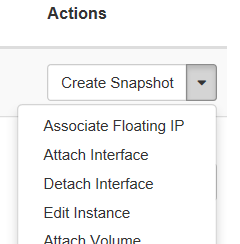
\includegraphics[scale=0.7]{img/associate_IP_1.png}
\end{center}
\item A pop-up window will appear and under IP Address select from the
  drop-down menu an IP address from the available pool.
\begin{center}
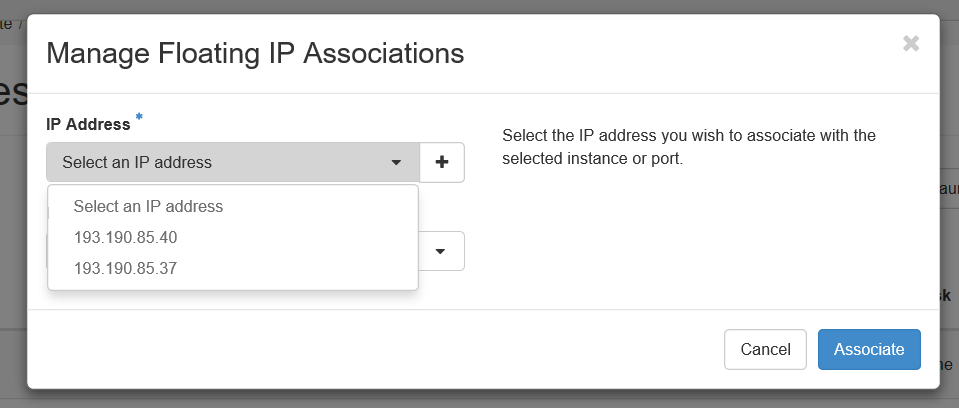
\includegraphics[scale=0.5]{img/associate_IP_2.png}
\end{center}
\item Click Associate
\end{enumerate}

If the IP has been successfully associated in the upper right corner of the browser screen will appear a green confirmation. If not successful a red notification will pop up that something went wrong.

\strong{Note:} To disassociate an IP address from an instance, click
the Disassociate button in the Actions column.

% TODO: remove this warning once we've removed the "Release Floating
% IP" buttons from the dashboard.
\strong{Warning:} \emph{Do not} use the Release Floating IP option in
the Actions column or on the overview page.  This will remove the
floating IP from the pool assigned to your project, something which
you, as a regular user, cannot undo.  If you've accidentally released
a floating IP, contact \cloudinfo to have it restored.

%%% Local Variables:
%%% mode: latex
%%% TeX-master: "intro-Cloud"
%%% End:


\chapter{Launch and manage instances}\label{cha:launch-manage-inst}
Instances are virtual machines that run inside the cloud. You can launch
an \gls{instance} from the following sources:

\begin{itemize}
\item Images uploaded to the Image service.

  \strong{Note:} Because images are read-only, any changes made while
  the instance is running will be lost when the instance is deleted,
  unless you choose to create a persistent volume for your instance
  when you launch it.  Using a volume, the VM's state is saved, even
  when the current instance is deleted.
\item Images which you previously copied to a persistent volume. The
  instance launches from the volume.
\item Instance snapshots.
\end{itemize}

\section{Launch an instance}\label{launch-an-instance}
\begin{enumerate}
\item Open the Compute tab and select the Instances category.

  The dashboard shows the list of existing instances with their name,
  IP addresses, flavor, status, power state, \ldots
\item Click \strong{Launch Instance}.
\item In the Launch Instance dialog box, specify the following values:

  \begin{center}
    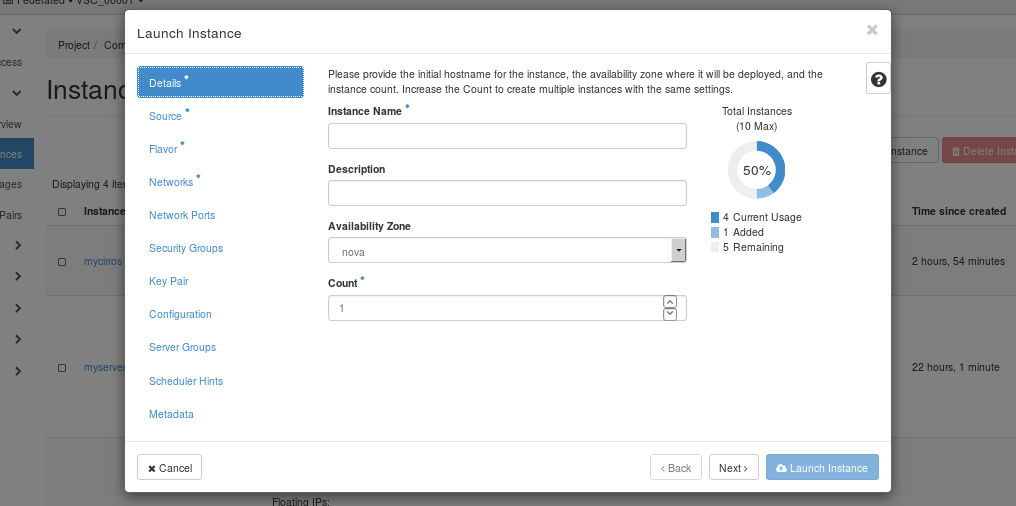
\includegraphics[scale=0.5]{img/tab-compute-instances-launch.png}
  \end{center}
  
  \begin{description}
  \item[Details] tab
    \begin{description}
    \item[Instance Name] Assign a name to the virtual machine.

      \strong{Note:} The name you assign here becomes the initial host
      name of the server. If the name is longer than 63 characters,
      the Compute service truncates it automatically to ensure dnsmasq
      works correctly.

      After the server is built, if you change the server name in the
      API or change the host name directly, the names are not updated
      in the dashboard.

      Server names are not guaranteed to be unique when created so you
      could have two instances with the same host name.

    \item[Description] You can assign a brief description of the
      virtual machine.
    \item[Availability Zone] Large-scale OpenStack systems may consist
      of multiple availability zones, which are groups of hypervisors
      connected to different power sources. By assigning instances to
      different availability zones, users can protect themselves
      against power failures.  However, the VSC cloud consists of just
      a single zone, called \strong{nova}.
    \item[Count] To launch multiple instances, enter a value greater
      than \strong{1}. The default is \strong{1}.
    \end{description}

    \begin{center}
      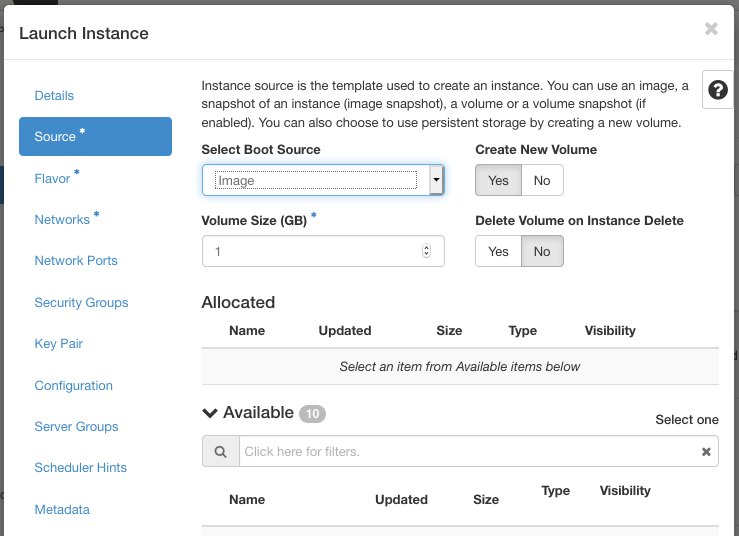
\includegraphics[width=0.7\textwidth]{img/launch_instance_source}
    \end{center}
  \item[Source] tab
  \begin{description}
  \item[Select Boot Source] Your options are:
    \begin{description}
    \item[Image]
    \item[Image snapshot]
    \item[Volume]
    \item[Volume snapshot]
    \end{description}
    Depending on the type of boot source, the list of available items
    changes.

  \item[Create New Volume] If you enable this option when launching
    from an image or instance snapshot, the image or snapshot will be
    copied to a volume.  This way, the state of your instance persists
    after shutdown and reboot.
  \end{description}

\item[Flavor] tab. Specify the size of the instance to launch.

  \strong{Note:} The flavor is selected based on the size of the image
  selected for launching an instance. For example, while creating an
  image, if you have entered the value in the Minimum RAM (MB) field
  as 2048, then on selecting the image, the default flavor is
  \strong{m1.small}.  If a `!' warning sign is displayed next to a
  resource for one of the flavors, that means that this flavor would
  exceed the project's quota for that resource, and therefore is not
  available.

\item[Networks] tab. Add one or more networks to the instance.

\item[Network Ports] tab. Activate the ports that you want to assign to
  the instance.
\item[Security Groups] tab. Activate the security groups that you want
  to assign to the instance.

  Security groups are a kind of cloud firewall that define which
  incoming network traffic is forwarded to instances.  See section
  \ref{cha:conf-access-secur} on page ~\pageref{sec:security-groups}
  for more information.

  The default security group is assigned to the instance
  automatically.
\item[Key Pair] tab. Specify a key pair.

  If the image uses a static root password or a static key set
  (neither is recommended), you do not need to provide a key pair to
  launch the instance.
\item[Configuration] tab. Specify a customization script that runs
  after your instance launches.

\item[Server Groups] tab.  You can organize instances into groups with
  a scheduling policy.  With an ``affinity'' policy, OpenStack will
  try to schedule those instances on the same hypervisors, which is
  useful for instances that need to communicate with each other a lot.
  With an ``anti-affinity'' policy, instances will be scheduled on
  different hypervisors, which you might use for instances that
  provide redundant copies of a single service.

\item[Scheduler Hints] tab.  By providing scheduler hints, you can get
  more fine grained control over which hypervisor your instances are
  scheduled on.

\item[Metadata] tab. Add Metadata items to your instance.
\end{description}

\item Click \strong{Launch Instance}.
\end{enumerate}

The instance starts on a compute node in the cloud.

\strong{Note:} If you did not provide a key pair, security groups, or
rules, users can access the instance only from inside the cloud
through VNC. Even pinging the instance is not possible without an ICMP
rule configured.

You can also launch an instance from the Images or Volumes category when
you launch an instance from an image or a volume respectively.

When you launch an instance from an image, OpenStack creates a local
copy of the image on the compute node where the instance starts.

For details on creating images, see
\href{https://docs.openstack.org/image-guide/create-images-manually.html}{\emph{Creating
images manually}} in the \emph{OpenStack Virtual Machine Image Guide}.

\section{Connect to an instance using SSH}\label{connect-to-your-instance-using-ssh}
Before you can connect to an instance using SSH, you must set up a
floating IP for it, as discussed in section~\ref{sec:floating-ip}.
Recall that only ports 50000 to 60000 of the floating IP's can be
directly reached from outside the UGent network.

\strong{Note:} When you try to connect to a new instance using a port
that was previously forwarded to a different instance --- either due
to a change in the port forwarding configuration, or because an old
instance was deleted and replaced --- your SSH client will show an
error message because the ``host key'' of the new instance doesn't
match the known previous key.  Section \nameref{sec:host-keys}
explains how to handle such errors.

\strong{Note:} If you want to access ports outside the public range,
you'll need to connect to the UGent login node
\lstinline{login.hpc.ugent.be} first, and hop to your instance from
there.  To make this work without storing the required private key for
the instance in your VSC storage space, you need to set up an SSH
agent with key forwarding locally, i.e.\ on the machine where you
store the private key of an authorized keypair for the instance.
Section 2.1.4 of the HPC introduction explains how to set this up
(\href{https://hpcugent.github.io/vsc\_user\_docs}{hpcugent.github.io/vsc\_user\_docs}).

\begin{enumerate}
  \setcounter{enumi}{-1}
\item (\emph{Only if using a port blocked by the UGent firewall, see
    the note above:}) Use your VSC account to connect to the UGent login
  node, using the \lstinline{ssh -A} option to enable agent
  forwarding:

  \begin{prompt}
    %\shellcmd{ssh -A vsc12345@login.hpc.ugent.be}
  \end{prompt}

\item Copy the address of the floating IP where your instance can be
  reached.  In our example, the address is 193.190.85.40.

\item Connect to the instance.  Use OpenSSH's \lstinline{-p} option to
  specify the port where the instance's SSH server can be reached,
  e.g. for port 50022:

  \begin{prompt}
    %\shellcmd{ssh -p 50022 ubuntu@193.190.85.40}
  \end{prompt}

  When you run the above command, your SSH client may display warnings
  or error messages.  The section \nameref{sec:host-keys}
  explains the meaning of these messages and how you should deal with
  them.

  \strong{Note:} The images we provide do not allow SSH logins for the
  root user.  There is a default user instead, who can get
  administrative privileges using \lstinline{sudo}.  In our example,
  we have used the username \lstinline{ubuntu} for Ubuntu images.
  Attempting to log in as root will return an error message with the
  proper user name.
\end{enumerate}

\subsection*{Host keys}\label{sec:host-keys}
When connecting to instances using SSH, you will sometimes see
warnings or errors related to ``host keys''.  This section briefly
explains the meaning of those errors, and how to deal with them.

When you try to connect to an instance, you use the private key of
your SSH keypair to prove your identity to that instance.  If you do
not have access to the right secret key, you can not prove your
identity, at which point the your instance's SSH server will deny
access.  In the same way, the server must prove its own identity to
you, using its own keypair or ``host key''.  Without such a
verification procedure, third parties on the network between you and
the instance could perform a so-called man-in-the-middle-attack, where
they intercept the communication between you and the server you want
to reach and steal valuable information.

To prevent such man-in-the-middle attacks, the SSH client on your
system stores the host key for every IP address you have connected to,
and verifies the key the next time you try to connect to that address.
If all goes well, this check is silently performed in the background,
but there are a number of situations where the check fails.  In this
case, you have to look up the host key of your instance in the
OpenStack dashboard to verify that the connection is secure.

\subsubsection*{Looking up an instance's host
  key}\label{sec:look-up-hostkey}
In order to verify a host key, it suffices to compare the key's
fingerprint, a short alphanumerical sequence computed from the keys
content.  You can use the Dashboard to look up the host key
fingerprint for an instance as follows:
\begin{enumerate}
\item Open the Compute tab and select the Instances category.
\item Click on the name of the instance you want to connect to.
\item Click \strong{Log}
  \begin{center}
    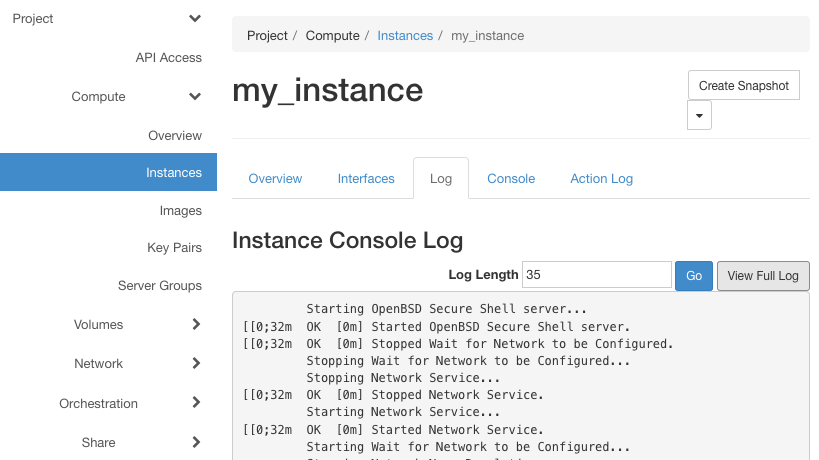
\includegraphics[width=0.8\textwidth]{img/instance_log}
  \end{center}

\item Click \strong{View Full Log}.  You are taken to a new page with a long text listing.
\item Search for the words \lstinline{-----BEGIN SSH HOST KEY FINGERPRINTS-----} to find the log file section containing the host key fingerprints, for example:
\begin{code}{}
<14>Jun  6 09:57:01 ec2: #############################################################
<14>Jun  6 09:57:01 ec2: -----BEGIN SSH HOST KEY FINGERPRINTS-----
<14>Jun  6 09:57:01 ec2: 1024 SHA256:gCa0hZAaOnpzxYM5WnAZINuZTI5NAoqd41U/dtxeGKE root@my-instance (DSA)
<14>Jun  6 09:57:01 ec2: 256 SHA256:nyujUIF37c674FPSkDdz0xgAU6S39UWbmMzBPmdmCmg root@my-instance (ECDSA)
<14>Jun  6 09:57:01 ec2: 256 SHA256:Mcznquek1A3BFz6KEXSxsivpdkX1mY3LnymEA7C8Xxg root@my-instance (ED25519)
<14>Jun  6 09:57:01 ec2: 2048 SHA256:4DagYc9cZvANkSjbTL0pB+3ULqHg09zW4E8wvDrB4Do root@my-instance (RSA)
<14>Jun  6 09:57:01 ec2: -----END SSH HOST KEY FINGERPRINTS-----
<14>Jun  6 09:57:01 ec2: #############################################################
\end{code}
\end{enumerate}

In this example, the fingerprints are character sequences starting
with ``SHA256'', such as the ECDSA key fingerprint
\lstinline{SHA256:nyujUIF37c674FPSkDdz0xgAU6S39UWbmMzBPmdmCmg}.  The
following sections describe the most common cases where you'll need
these fingerprints.

\strong{Note:} The following examples show output and commands for
OpenSSH, the most common client on Linux and macOS.  If you are
working from a windows system using using PuTTY, we refer to sections
8.4 and 8.6 of the windows version of the
\href{https://hpcugent.github.io/vsc\_user\_docs}{introduction to
  HPC} for the corresponding warning messages.

\subsubsection*{Connecting for the first time}\label{sec:conn-first-time}
The first time you connect to a new ip address:port combination, your SSH client does not know the host key for this address, and therefore it can't verify the identity of the server.  When using OpenSSH, the warning looks as follows (again using address 193.190.85.40 and port 50022 as an example):

\begin{prompt}
The authenticity of host '[193.190.85.40]:50022 ([193.190.85.40]:50022)'
can't be established.
ECDSA key fingerprint is SHA256:nyujUIF37c674FPSkDdz0xgAU6S39UWbmMzBPmdmCmg.
Are you sure you want to continue connecting (yes/no)?
\end{prompt}

Verify the fingerprint in order to make sure that it is safe to
proceed:

\begin{enumerate}
\item Look up the fingerprint of the instance you want to access,
  according to the procedure described in the section
  \nameref{sec:look-up-hostkey}.
\item Verify that the fingerprint you find in the Dashboard matches
  the fingerprint shown in the warning message.

  In this example, we see that the ECDSA key fingerprint reported by
  the SSH client matches the fingerprint of our instance from the
  previous section, namely

  \lstinline{SHA256:nyujUIF37c674FPSkDdz0xgAU6S39UWbmMzBPmdmCmg}.

\item If the fingerprints are identical, type ``yes'' to log in.
  \strong{If the fingerprints do not match, type ``no'', and contact
    \cloudinfo.}
\end{enumerate}

\subsubsection{New instance at a known address}
Another case where the host key verification fails, is when you try to access a new instance at an IP address and port previously used by another instance.  This can happen if you modify your port forwarding configuration, or if a running instance connected to a certain port is deleted and replaced by a new one.  In this case, OpenSSH will show a warning such as this:

\begin{prompt}
@@@@@@@@@@@@@@@@@@@@@@@@@@@@@@@@@@@@@@@@@@@@@@@@@@@@@@@@@@@
@    WARNING: REMOTE HOST IDENTIFICATION HAS CHANGED!     @
@@@@@@@@@@@@@@@@@@@@@@@@@@@@@@@@@@@@@@@@@@@@@@@@@@@@@@@@@@@
IT IS POSSIBLE THAT SOMEONE IS DOING SOMETHING NASTY!
Someone could be eavesdropping on you right now (man-in-the-middle attack)!
It is also possible that a host key has just been changed.
The fingerprint for the ECDSA key sent by the remote host is
SHA256:hI2HcqFxsCKwEauq2QvBmgDN4nCPjllaRsYoCb7tJQw.
Please contact your system administrator.
Add correct host key in [...]/.ssh/known_hosts to get rid of this message.
Offending ECDSA key in [...]/.ssh/known_hosts:57
ECDSA host key for [193.190.85.40]:50322 has changed and you have requested strict checking.
Host key verification failed.
\end{prompt}

The file \lstinline{known_hosts} in your OpenSSH configuration
directory contains a list of all hosts you have previously connected
to, together with their host keys.  The warning above tells you that
the server you are connecting to is not using the same key anymore.
In this case, you should take the following steps:
\begin{enumerate}
\item Look up the fingerprint of the instance you want to access,
  according to the procedure described in the section
  \nameref{sec:look-up-hostkey}.
\item Verify that the fingerprint you find in the Dashboard matches
  the fingerprint shown in the warning message.
\item If the fingerprint matches, the new key is legitimate. Remove
  the previous known key from the \lstinline{known_hosts} file as
  follows (still using address 193.190.85.40 and port number 50322 as
  an example):

  \begin{prompt}
    % \shellcmd{ssh-keygen -R [193.190.85.40]:50322}%\end{prompt}

    This command causes OpenSSH to forget the previous key.  On your
    next attempt to connect to that address, OpenSSH will treat it as
    a new host and ask you to verify the fingerprint as described in
    section \nameref{sec:conn-first-time}.

  \strong{If the fingerprint does not match, do not attempt to connect, and contact \cloudinfo.}
\end{enumerate}

\section{Track usage for instances}\label{track-usage-for-instances}

You can track usage for instances for each project. You can track costs
per month by showing meters like number of vCPUs, disks, RAM, and uptime
for all your instances.

\begin{enumerate}
\item Open the Compute tab and select the Overview category.
\item To query the instance usage for a period of time, select a time
  range and click \strong{Submit}.
\item To download a summary, click \strong{Download CSV Summary}.
\end{enumerate}

\section{Create an instance snapshot}\label{create-an-instance-snapshot}

\begin{enumerate}
\item Open the Compute tab and select the Instances category.
\item Select the instance from which to create a snapshot.
\item In the actions column, click \strong{Create Snapshot}.
\item In the Create Snapshot dialog box, enter a name for the snapshot, and
  click \strong{Create Snapshot}.
\end{enumerate}

The Images category shows the instance snapshot.

To launch an instance from the snapshot, select the snapshot and click
Launch. Proceed with launching an instance.

\section{Manage an instance}\label{manage-an-instance}

\begin{enumerate}
\item Open the Compute tab and select the Instances category.
\item Select an instance.
\item In the menu list in the actions column, select the state.

  You can resize or rebuild an instance. You can also choose to view
  the instance console log, edit instance or the security
  groups. Depending on the current state of the instance, you can
  pause, resume, suspend, soft or hard reboot, or terminate it.
\end{enumerate}

\subsection*{Difference between \emph{suspend}, \emph{pause}, \emph{shelve}, \emph{shut off}, \emph{delete}}\label{server-power-down-states}

\begin{description}
\item[Pause] Stores the state of the VM in the (RAM) memory.
\item[Suspend] Stores the state of the VM on the disk, all memory is
  written to disk, and the server is stopped.
\item[Shut off] The server is powered down by the user, either through
  the OpenStack Compute API, or from within the server by issuing a
  \emph{shutdown -h} command. In this state the user retains all
  computational resources associated with the VM. The instance can be
  later restarted.
\item[Shelve] Shelving stops the instance and takes a snapshot of
  it. Then depending on the value of the \emph{shelved\_offload\_time}
  config option, the instance is either deleted from the hypervisor
  (0), never deleted (-1), or deleted after some period of time (>
  0). Shelve preserves all associated data and VM resources but does
  not retain anything in memory.
\item[Delete] The VM is deleted and removed from \gls{OpenStack}
  together with any associated processes and resources.  However, for
  instances backed by a persistent volume, this volume is not deleted.
  When such an instance is deleted, you can restore it by launching a
  new instance from the volume, or delete the volume as well (see
  section \ref{delete-a-volume}).
\end{description}

For more details see the OpenStack documentation on \href{https://docs.openstack.org/nova/\osversion/reference/vm-states.html}{\emph{Virtual Machine States and Transitions}} and \href{https://developer.openstack.org/api-guide/compute/server_concepts.html}{\emph{Server concepts}}.

%%% Local Variables:
%%% mode: latex
%%% TeX-master: "intro-Cloud"
%%% End:


\chapter{Create and manage volumes}
An \gls{OpenStack Volume} is a block storage device which you attach
to instances to enable persistent storage. You can attach a volume to
a running instance or detach a volume and attach it to another
instance at any time. You can also create a snapshot from a volume, or
delete it.

\subsubsection{Create a volume}\label{create-a-volume}
\begin{enumerate}
\item Open the Volumes tab and select the Volumes category.
\item Click \strong{Create Volume}.

  In the dialog box that opens, enter or select the following values.

  \begin{description}
  \item[Volume Name] Specify a name for the volume.
  \item[Description] Optionally, provide a brief description for the volume.
  \item[Volume Source] Select one of the following options:

    \begin{itemize}
    \item No source, empty volume: Creates an empty volume. An empty
      volume does not contain a file system or a partition table.
    \item Snapshot: If you choose this option, a new field for Use
      snapshot as a source displays. You can select the snapshot from
      the list.
    \item Image: If you choose this option, a new field for Use image
      as a source displays. You can select the image from the list.
    \item Volume: If you choose this option, a new field for Use
      volume as a source displays. You can select the volume from the
      list. Options to use a snapshot or a volume as the source for a
      volume are displayed only if there are existing snapshots or
      volumes.
    \end{itemize}
  \item[Type] Leave this field blank.
  \item[Size (GB)] The size of the volume in gibibytes (GiB).
  \item[Availability Zone] Select the Availability Zone from the
    list. By default, this value is set to the availability zone given
    by the cloud provider (for example, \strong{us-west} or
    \strong{apac-south}). For some cases, it could be \strong{nova}.
  \end{description}
\item Click \strong{Create Volume}.
\end{enumerate}

The dashboard shows the volume on the Volumes tab.

\subsubsection{Attach a volume to an
  instance}\label{attach-a-volume-to-an-instance}
After you create one or more volumes, you can attach them to
instances.  You can attach a volume to one instance at a time.

\begin{enumerate}
\item Open the Volumes tab and click Volumes
  category.
\item Select the volume to add to an instance and click \strong{Manage
  Attachments}.
\item In the Manage Volume Attachments dialog box, select an instance.
\item Enter the name of the device from which the volume is accessible
  by the instance.

  \strong{Note:} The actual device name might differ from the volume
  name because of hypervisor settings.
\item Click \strong{Attach Volume}.

  The dashboard shows the instance to which the volume is now attached
  and the device name.
\end{enumerate}
You can view the status of a volume in the Volumes tab of the dashboard.
The volume is either Available or In-Use.

Now you can mount, format, and use the volume from this instance.

\subsubsection{Detach a volume from an instance}\label{detach-a-volume-from-an-instance}
\begin{enumerate}
\item Open the Volumes tab and select the Volumes category.
  \item Select the volume and click \strong{Manage Attachments}.
  \item Click \strong{Detach Volume} and confirm your changes.
  \end{enumerate}

A message indicates whether the action was successful.

\subsubsection{Create a snapshot from a
  volume}\label{create-a-snapshot-from-a-volume}
\begin{enumerate}
\item Open the Volumes tab and select the Volumes category.
\item Select a volume from which to create a snapshot.
\item In the Actions column, click \strong{Create Snapshot}.
\item In the dialog box that opens, enter a snapshot name and a brief
  description.
\item Confirm your changes.
\end{enumerate}

The dashboard shows the new volume snapshot in Volume Snapshots tab.

\subsubsection{Edit a volume}\label{edit-a-volume}
\begin{enumerate}
\def\labelenumi{\arabic{enumi}.}
\item Open the Volumes tab and select the Volumes category.
\item Select the volume that you want to edit.
\item In the Actions column, click \strong{Edit Volume}.
\item In the Edit Volume dialog box, update the name and description
  of the volume.
\item Click \strong{Edit Volume}.
\end{enumerate}

\strong{Note:} You can extend a volume by using the Extend Volume
option available in the More dropdown list and entering the new value
for volume size.

\subsubsection{Delete a volume}\label{delete-a-volume}
When you delete an instance, the data in its attached volumes is not
deleted.

\begin{enumerate}
\item Open the Volumes tab and select the Volumes category.
\item Select the check boxes for the volumes that you want to delete.
\item Click \strong{Delete Volumes} and confirm your choice.
\end{enumerate}

A message indicates whether the action was successful.

%%% Local Variables:
%%% mode: latex
%%% TeX-master: "intro-Cloud"
%%% End:


\chapter{Orchestration Using Heat}\label{cha:orch-using-heat}
\gls{Heat} is the name of the OpenStack orchestration engine, which
can manage complete configurations of all servers, volumes, users,
networks and routers that make up a cloud application.  Instead of
managing every component separately, we can create, start, stop or
clean up our complete application in a single step.  Such a set of
collectively managed resources is called a \gls{stack}.

\gls{Heat} has its own dashboard interface, which you can find under
the \strong{Orchestration} tab of the main OpenStack dashboard.  Official
documentation for Heat and its dashboard interface can be found at the
following locations:
\begin{itemize}
\item \url{https://docs.openstack.org/heat/\osversion}
\item \url{https://docs.openstack.org/heat-dashboard/\osversion}
\end{itemize}

\section{\gls{Heat Orchestration Template}s}\label{sec:glsh-orch-templ}
A \gls{stack}'s resources and their mutual dependencies can be
specified in a text file, called a \gls{Heat Orchestration Template}
(\textsc{hot}).  The syntax of these templates conforms to the
\gls{yaml} standard, for which many text editors provide specialized
editing modes.  The following example describes a stack consisting of
a single VM:
\begin{code}{}
heat_template_version: 2018-03-02

description: Deploy a single compute instance

parameters:
  user_network:
    type: string
    label: user_network
    description: Add the required VM network
    constraints: [ custom_constraint: neutron.network ]
  user_key:
    type: string
    label: ssh_user_key
    description: Public ssh key for user authentication
    constraints: [ custom_constraint: nova.keypair ]

resources:
  my_instance:
    type: OS::Nova::Server
    properties:
      security_groups: [ default ]
      networks: [ network: { get_param: user_network } ]
      key_name: { get_param: user_key }
      image: Ubuntu_16.04_2NICs
      flavor: m1.small
\end{code}

Our example contains four main sections:
\begin{description}
\item[\texttt{heat\_template\_version}] The \textsc{hot} specification
  has evolved since its initial release.  The key
  \lstinline{heat_template_version} indicates the version of the
  syntax used in this template.  It's value can be a release date or
  (in recent version) the name of the version.
\item[\texttt{description}] A description is optional, but
  recommended.
\item[\texttt{parameters}] An optional section, \lstinline{parameters}
  allow users to configure various properties when instantiating a new
  stack, without having to edit the template itself.  A parameter
  value can be used elsewhere in the template using the function
  \lstinline{get_param}.
\item[\texttt{resources}] This section contains all the resources used
  by the Stack.  In this case, there is just a single VM instance.
\end{description}
Optional additional sections are \strong{\lstinline{parameter_groups}},
\strong{\lstinline{outputs}}, and \strong{\lstinline{conditions}}.

The
`\href{https://docs.openstack.org/heat/\osversion/template_guide}{Template
  Guide}' in the Heat documentation contains a specification of the
\textsc{hot} format, as well as information on how to describe the
various types of resources in a template.  \textsc{vsc} also provides
some example templates in the repository
\url{https://github.com/hpcugent/openstack-templates}.

\section{The Template Generator}\label{sec:template-generator}
The Heat dashboard provides a graphical interface where users can draw
templates by dragging resources onto a canvas, and connecting them.
Users can then download a template generated from this interface, or
immediately instantiate it as a stack.

\subsubsection{Example: an instance with a public IP}
As an example, we will create a template for a single node attached to
a floating IP from the public pool, making it accessible from outside
the OpenStack cloud.  It might be useful to compare this approach to
that of the example
`\href{https://docs.openstack.org/heat/\osversion/template_guide/basic_resources.html#create-and-associate-a-floating-ip-to-an-instance}{Create
  and associate a floating IP to an instance}' in Heat Template Guide.

\begin{enumerate}
\item Open the \strong{Template Generator} from the
  \strong{Orchestration} tab.  Here, you are presented with a set of
  icons for the different resources, and a canvas.  The floppy disk
  icon (``Manage Drafts'') allows you to save and restore different
  versions of your work.
  \begin{center}
    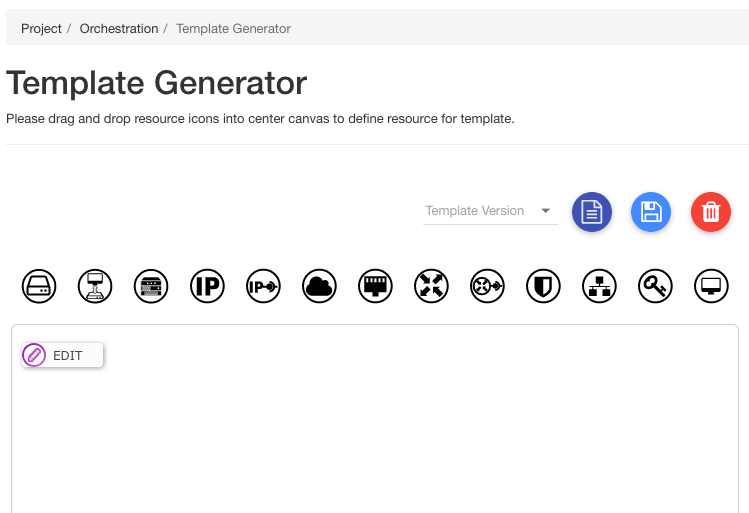
\includegraphics[width=0.7\textwidth]{img/template_generator}
  \end{center}
\item You can now drag and drop icons onto the canvas to add resources
  to the template.  Add a VM (OS::Nova::Server), a port
  (OS::Neutron::Port), a floating ip (OS::Neutron::FloatingIP), and a
  floating ip association (OS::Neutron::FloatingIPAssociation).
  \begin{center}
    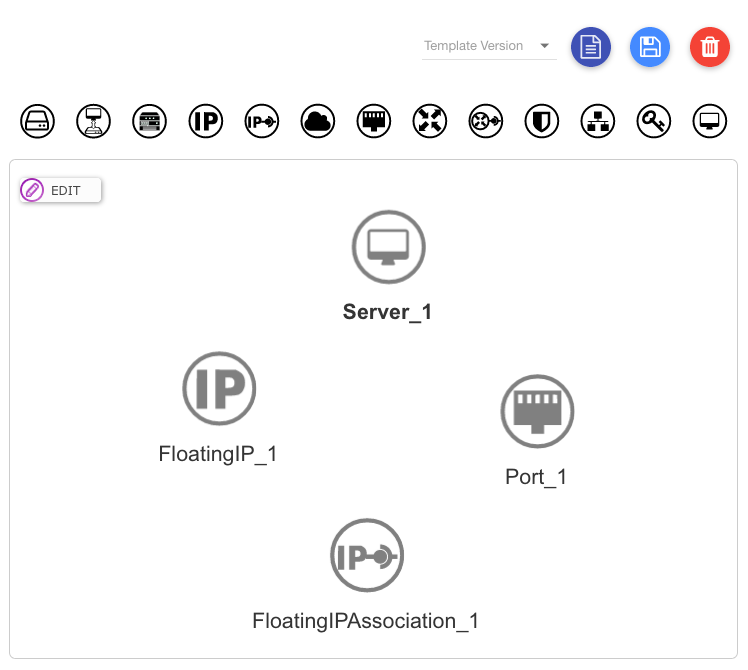
\includegraphics[width=0.7\textwidth]{img/all_resources}
  \end{center}
\item Associate the port to the server: click the purple
  \strong{\textsc{edit}} icon, select \strong{\textsc{add edge}}, and
  click and drag to draw an edge from Server\_1 to Port\_1.  This will
  make Port\_1 a port of Server\_1.  Note that edges are directed: the
  resource at the end-point of an edge becomes a property of the
  resource at the starting point.  You can't draw an edge from Port\_1
  to Server\_1.
  \begin{center}
    \includegraphics[width=0.7\textwidth]{img/draw_edge}
  \end{center}
\item In the same way, draw an edge from FloatingIPAssociation\_1 to
  Port\_1, and from FloatingIPAssociation\_1 to FloatingIP\_1.  The
  stack's graph should now look as follows:
  \begin{center}
    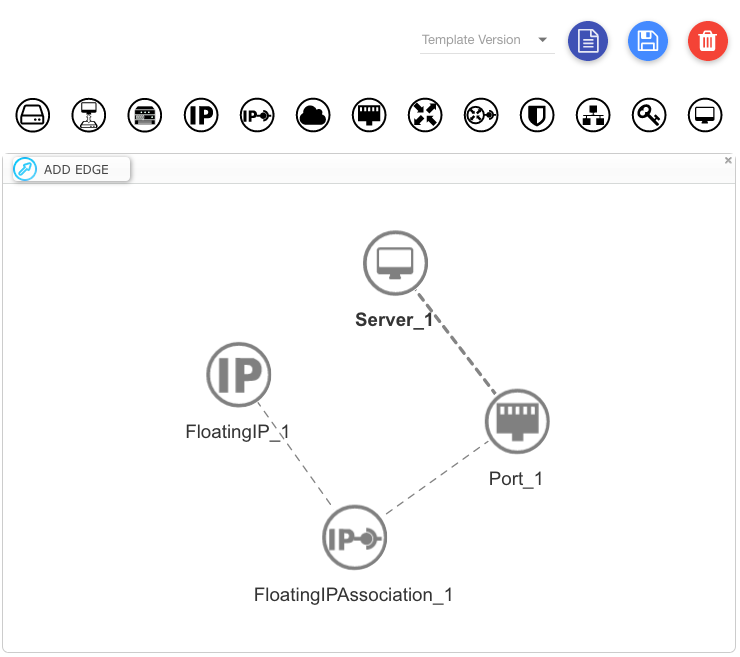
\includegraphics[width=0.7\textwidth]{img/all_resources_connected}
  \end{center}
\item Next, specify the required properties of each resource.
  Left-clicking a resource opens up a window with properties.
  \begin{itemize}
  \item For Server\_1, configure a VM flavor and boot source in the
    \strong{\textsc{basic}} tab.  In the \strong{\textsc{access \&
        security}} tab, select a public key for authentication.  You
    can also have a look at the \strong{\textsc{networks}} tab, where
    you should see the \strong{Port} property for Port\_1, which
    corresponds to the edge connecting Server\_1 to Port\_1.  Click
    \strong{\textsc{save}} to save your settings and close the
    property window.
    \begin{center}
      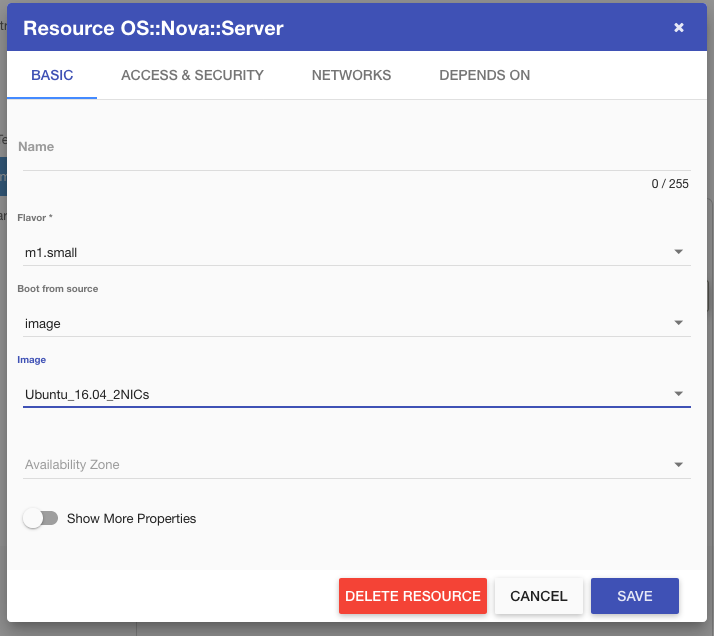
\includegraphics[width=0.7\textwidth]{img/server_basic_properties}
      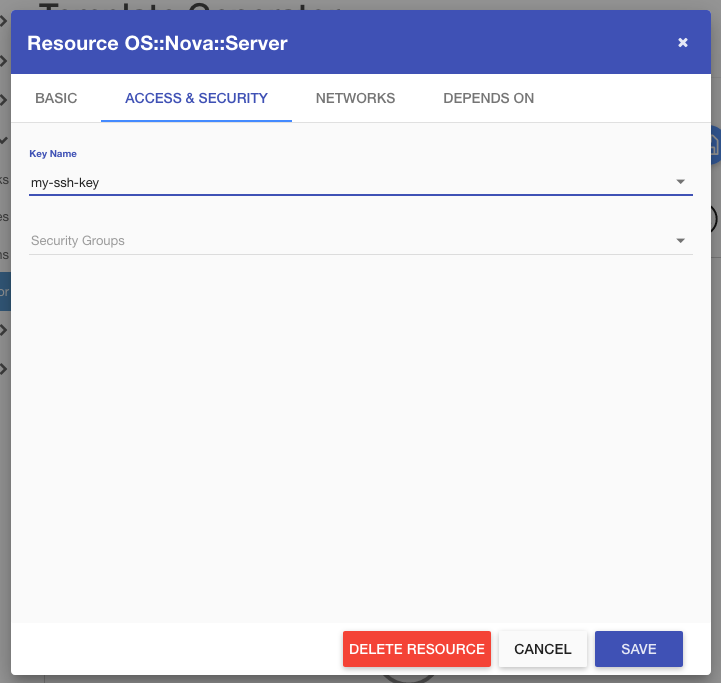
\includegraphics[width=0.7\textwidth]{img/server_access_security}
      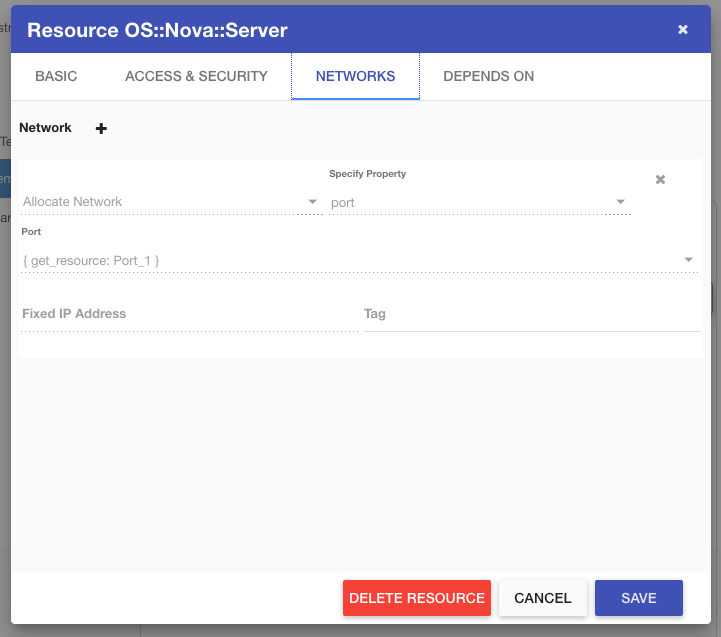
\includegraphics[width=0.7\textwidth]{img/server_networks}
    \end{center}
  \item In the properties for Port\_1, you should select the \emph{vm}
    network in \strong{Network}, enable at least the \emph{default} security
    group, and check \strong{Port Security Enabled}.  Click \strong{\textsc{save}}.
    \begin{center}
      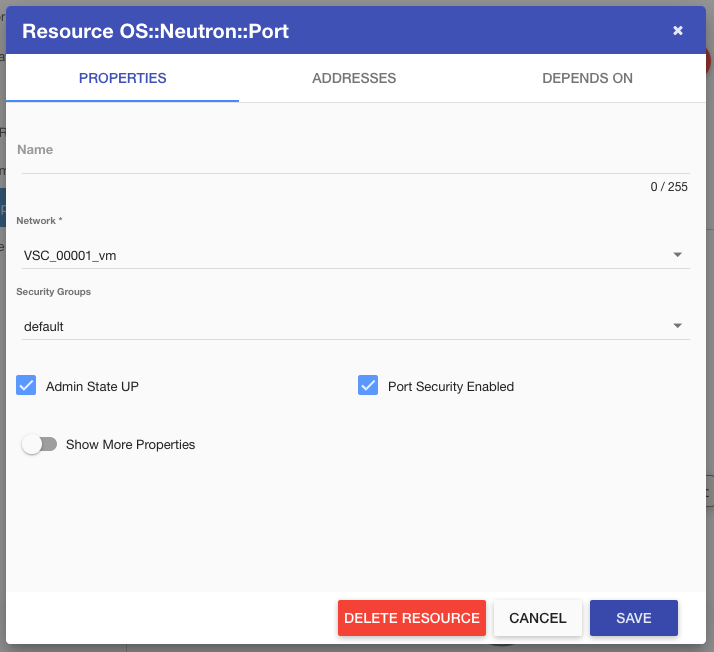
\includegraphics[width=0.7\textwidth]{img/port_properties}
    \end{center}
  \item Choose the network for FloatingIP\_1.  Select the \emph{public}
    network to obtain a public floating ip, which will allow outside
    access to your VM.  Click \strong{\textsc{save}}.
    \begin{center}
      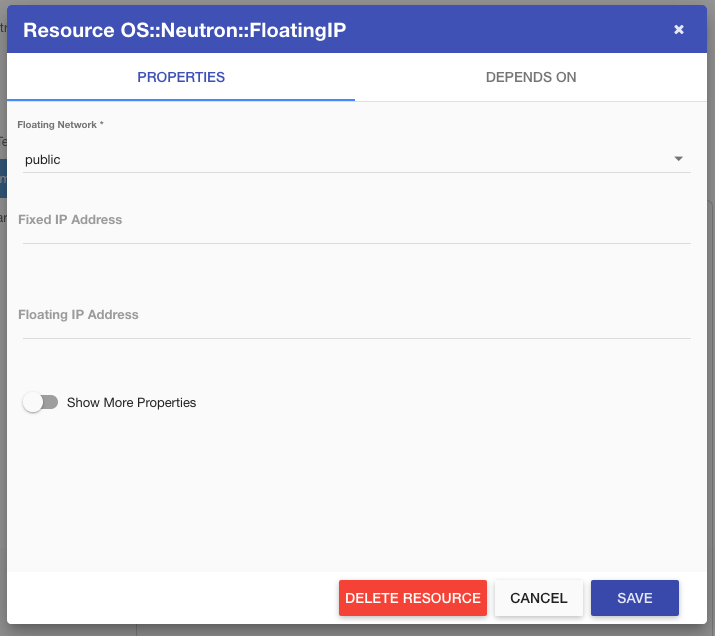
\includegraphics[width=0.7\textwidth]{img/floatingip_properties}
    \end{center}
  \item When you open up the properties window for
    FloatingIPAssociation\_1, you can see that the \strong{Floating
      IP} and \strong{Port ID} properties are set correctly, because
    edges connect FloatingIPAssociation\_1 to Port\_1 and
    FloatingIP\_1.  However, you still need to click
    \strong{\textsc{save}} in order to be able to generate a template
    from this configuration later on.
    \begin{center}
      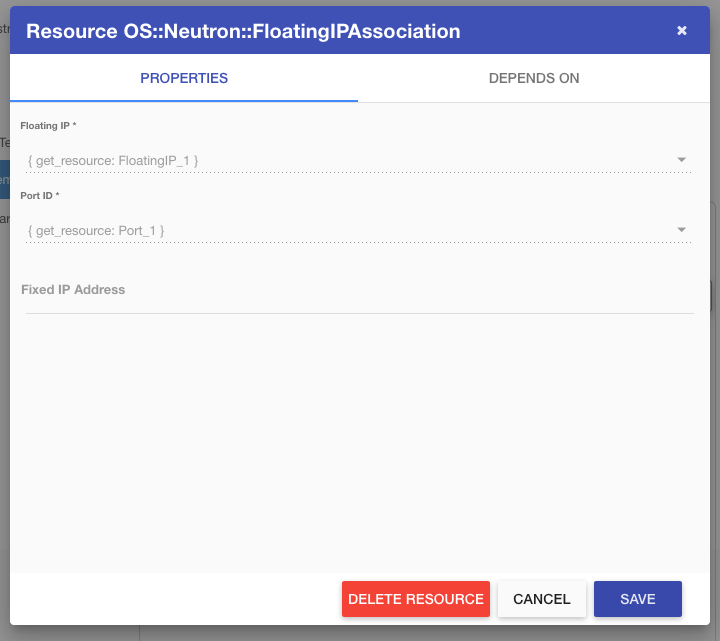
\includegraphics[width=0.7\textwidth]{img/floatingipassociation_properties}
    \end{center}
  \end{itemize}
\item When all required properties have been set and saved, the
  template's resources are drawn in a blue color.  We are now ready to
  generate a template from our configuration.
  \begin{center}
    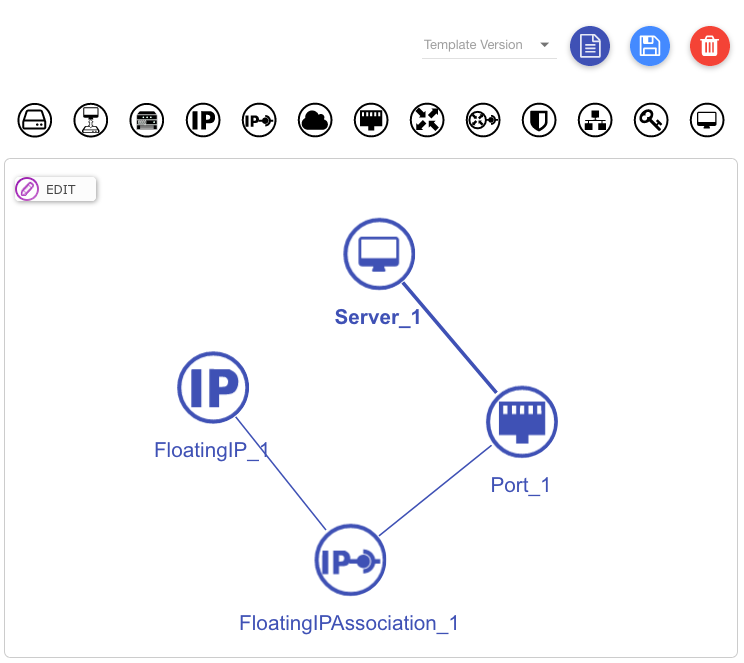
\includegraphics[width=0.7\textwidth]{img/stack_complete}
  \end{center}
\item In the \strong{Template Version} drop-down menu, select the
  version of the \textsc{hot} syntax you wish to use, e.g.\
  \emph{heat\_template\_version.2018-03-02}.  Now you can click the
  document icon to see the generated template, which you can download,
  or immediately instantiate using \strong{\textsc{create stack}}.
  \strong{Note:} \strong{\textsc{create stack}} takes you out of the
  template generator, with no option to resume working on the
  configuration, unless you save a draft first.
  \begin{center}
    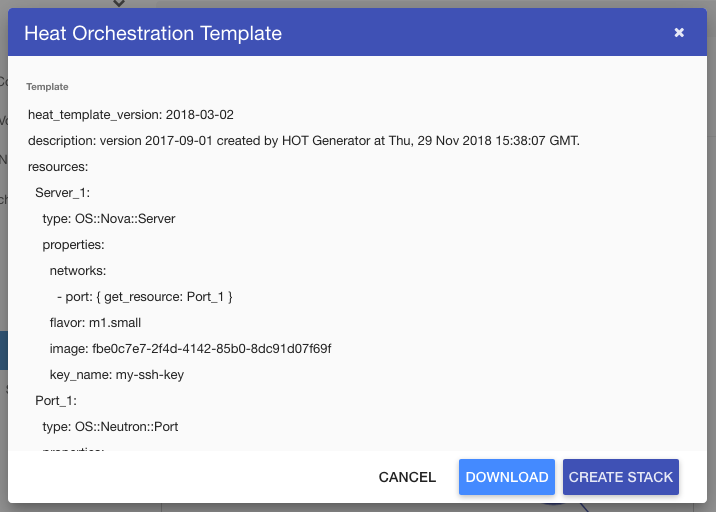
\includegraphics[width=0.7\textwidth]{img/complete_template}
  \end{center}
\end{enumerate}

The resulting template should look as follows:

\begin{code}{}
heat_template_version: 2018-03-02
description: version 2017-09-01 created by HOT Generator at Wed, 28 Nov 2018 13:45:30 GMT.
resources:
  FloatingIP_1:
    type: OS::Neutron::FloatingIP
    properties:
      floating_network: fc06776a-02df-4962-8513-aea8b8177fd2
  FloatingIPAssociation_1:
    type: OS::Neutron::FloatingIPAssociation
    properties:
      floatingip_id: { get_resource: FloatingIP_1 }
      port_id: { get_resource: Port_1 }
  Port_1:
    type: OS::Neutron::Port
    properties:
      admin_state_up: true
      security_groups:
        - 462946d4-aec5-400c-848b-edd916760b25
      network: 2a6d5e54-91b9-4e47-8692-409f4ce1e1c8
      port_security_enabled: true
  Server_1:
    type: OS::Nova::Server
    properties:
      networks:
        - port: { get_resource: Port_1 }
      flavor: m1.small
      image: fbe0c7e7-2f4d-4142-85b0-8dc91d07f69f
      key_name: my-ssh-key
\end{code}

Some resource types, such as shares, and some features of OpenStack
templates, such as template parameters, are not available in the
template generator, but a generated template can serve as a starting
point for more advanced configurations.

\section{Managing stacks}\label{sec:managing-stacks}
The \strong{Stacks} button in the \strong{Orchestration} tab takes you
to the overview page where you can launch, suspend, resume and delete
stacks.
\begin{center}
  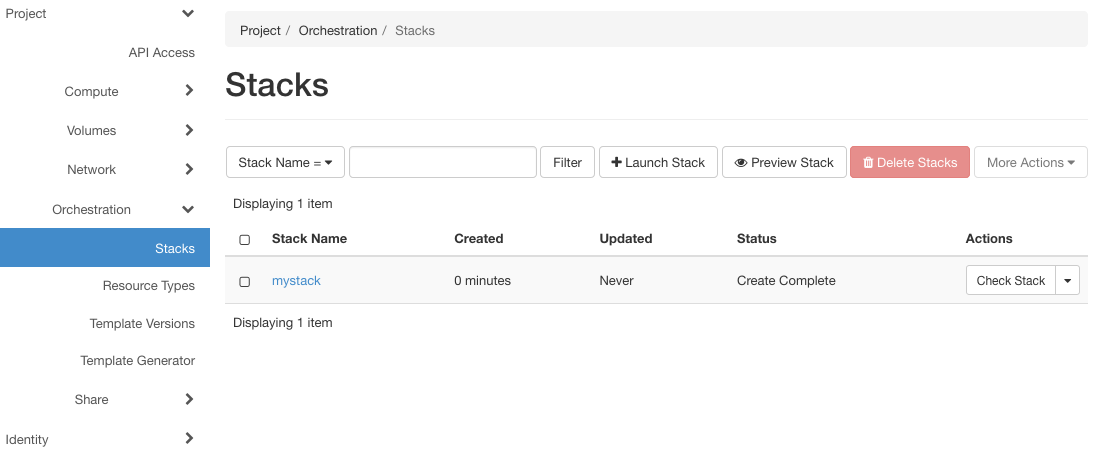
\includegraphics[width=\textwidth]{img/stacks_overview}
\end{center}
The overview page contains a list of all currently existing stacks
(either running or suspended), and buttons to perform the following
actions:

\begin{description}
\item{\strong{Launch Stack}} starts a wizard to create a stack from a
  template.  Depending on your choice of \strong{Template Source}, you
  can provide a local file on your system, directly type (or paste)
  the template text, or enter a \textsc{url} to download a template
  from that location.  You can also immediately launch a stack from
  the template generator (see section \ref{sec:template-generator})
  using the button \strong{\textsc{create stack}}.
\item{\strong{Preview Stack}} starts a similar wizard, but only
  performs a sanity check of your template, without instantiating the
  stack.  If the check passes, you can inspect the parameters of the
  stack that would be created.  The wizard does not allow you to enter
  input parameter values, so any mandatory input parameters should be
  provided in an environment (see
  `\href{https://docs.openstack.org/heat/\osversion/template_guide/environment.html}{Environments}'
  in the Heat template guide).
\item{\strong{Delete Stacks}} deletes the marked stacks.  Beware that
  deleting a stack also deletes all of a stack's physical resources,
  unless a different policy was set in the
  \strong{\lstinline{deletion\_policy}} property for those resources
  (see the item
  `\href{https://docs.openstack.org/heat/\osversion/template_guide/hot_spec.html#resources-section}{Resources
    section}' in the \textsc{hot} specification).
\item{\strong{More Actions}} hides the following additional actions:
  \begin{description}
  \item{\strong{Check Stacks}} verifies if the resources for selected
    stacks are still running.
  \item{\strong{Suspend Stacks}} suspends all resources of the
    selected stacks.
  \item{\strong{Resume Stacks}} resumes the selected (suspended) stacks.
  \end{description}
\end{description}
You can quickly suspend, resume or delete a single stack using the
drop-down menu in the \strong{Actions} column of the overview.  This
menu also contains the option \strong{Change Stack Template}, which
allows you to update a Stack by providing a new template.

\subsubsection{Example: launching a stack}
We can instantiate one of the examples from the \textsc{vsc}
repository \url{https://github.com/hpcugent/openstack-templates} by
providing a ``raw'' Github url:
\begin{center}
  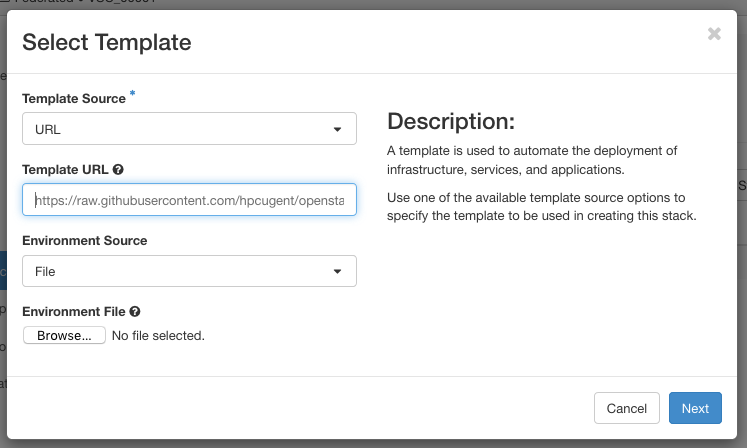
\includegraphics[width=0.7\textwidth]{img/launch_stack_template}
\end{center}
If the template uses parameters, we can specify their values on the
next page of the wizard.  In our example, \strong{nfs\_mount\_point},
\strong{ssh\_user\_key} and \strong{user\_network} are the template
parameters.
\begin{center}
  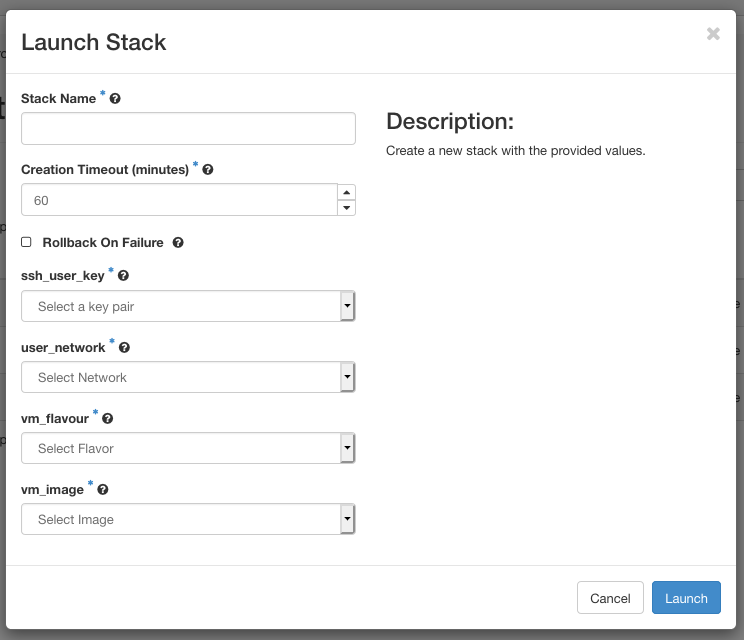
\includegraphics[width=0.7\textwidth]{img/launch_stack_parameters}
\end{center}
Finally, press the Launch button to create the stack.

%%% Local Variables:
%%% mode: latex
%%% TeX-master: "intro-OpenStack"
%%% End:


\chapter{Orchestration Using Terraform}\label{cha:orch-using-terraform}

HashiCorp \gls{Terraform} \url{https://www.terraform.io/} is an infrastructure
as code tool (IaC), similar to OpenStack \gls{Heat} orchestrator (\ref{cha:orch-using-heat}).
Users can deploy a data center infrastructure using a declarative
configuration language known as HashiCorp Configuration Language (HCL), or using JSON.
\gls{Terraform} has some advantages over OpenStack \gls{Heat} service.
It is has a simple syntax, it can provision virtual infrastructures across multiple cloud
providers (not only OpenStack) and it provides important features not supported
by \gls{Heat} at this moment, like network port forwarding rules (see \ref{sec:floating-ip}).
This means with Terraform scripts like \lstinline{neutron_port_forward}
(see \ref{port-forwarding}) are not longer needed.

The user can use \gls{Terraform} to deploy all the infrastructure and network rules from scratch.

It is currently one of the most popular infrastructure automation tools available.
VSC Cloud also provides some template examples that could be used to deploy virtual
infrastructures within VSC Tier-1 Cloud in an automated way
(\url{https://github.com/hpcugent/openstack-templates/tree/master/terraform}).

\gls{Terraform} client is available for different Operating Systems like Windows,
Linux or macOS (\url{https://www.terraform.io/downloads}) but it is also available from
UGent login node \lstinline{login.hpc.ugent.be}.

\section{Create application credentials for Terraform}\label{sec:app-cred-terraform}

\gls{Terraform} uses OpenStack application credentials to authenticate
to VSC Cloud Tier-1 public API. It is a good practice to generate a new Application Credential
just to be used with \gls{Terraform} framework. The process is the same described in section \ref{sec:appl-cred}.

\strong{Note:} Make sure you download the new application credential as yaml file instead of openrc.

At this point you should have a clouds.yaml text file with these lines:
\begin{code}{}
# This is a clouds.yaml file, which can be used by OpenStack tools as a source
# of configuration on how to connect to a cloud. If this is your only cloud,
# just put this file in ~/.config/openstack/clouds.yaml and tools like
# python-openstackclient will just work with no further config. (You will need
# to add your password to the auth section)
# If you have more than one cloud account, add the cloud entry to the clouds
# section of your existing file and you can refer to them by name with
# OS_CLOUD=openstack or --os-cloud=openstack
clouds:
  openstack:
    
    auth:
      
      auth_url: https://cloud.vscentrum.be:13000
      
      application_credential_id: "xxxxxxxxxxxxxxxxxxxxxxxxx"
      application_credential_secret: "xxxxxxxxxxxxxxxxxxxxx"
    
      
        
    region_name: "regionOne"
        
      
    interface: "public"
    identity_api_version: 3
    auth_type: "v3applicationcredential"
\end{code}

As the file comments state, you should copy the current clouds.yaml to your VSC login node \$home
\lstinline{login.hpc.ugent.be}: \texttt{\emph{\~\//.config/openstack/clouds.yaml}}, or locally
if you have installed \gls{Terraform} in your own laptop or computer.
\gls{Terraform} will use this file to authenticate to OpenStack API automatically.


\section{Getting Terraform examples}\label{sec:getting-terraform-templ}

You can connect to UGent login node \lstinline{login.hpc.ugent.be} to use terraform.
Login to the login node with your VSC account first:

\begin{prompt}
%\shellcmd{ssh -A vscxxxxx@login.hpc.ugent.be}
\end{prompt}

If this is the first time using Terraform, download the VSC Terraform examples from github from
\url{https://github.com/hpcugent/openstack-templates}:

\begin{prompt}
%\shellcmd{git clone https://github.com/hpcugent/openstack-templates}
\end{prompt}

Make sure you have \texttt{\emph{\~\//.config/openstack/clouds.yaml}} available from the login node (see previous section \ref{sec:app-cred-terraform}).

\strong{Note:} Do not share your application credential file clouds.yaml or put this file in a public place.

\begin{prompt}
%\shellcmd{chmod 600 ~/.config/openstack/clouds.yaml}
\end{prompt}

\section{Generate Terraform template variables}\label{sec:generate-terraform-variables}
\gls{Terraform} requires some variables to know which resources are avaiable from the cloud provider for the user or project.
You do not have to include these variables manually, we have included a script to gather these variable IDs automatically.
From Terraform directory cloned from git in the previous step (see: \ref{sec:getting-terraform-templ}), got to scripts directory:

\begin{prompt}
%\shellcmd{cd ~/openstack-templates/terraform/scripts}
\end{prompt}

And now run the script (usually you only have to run this script once).

\begin{prompt}
%\shellcmd{./modify\_variable.sh}
\end{prompt}

This step will take some seconds. The script will contact to VSC OpenStack public API to gather all the resources available for your project and fetch all the resource's IDs.
Usually you only have to run this script once, unless something was changed/updated for your project's resources (like a new network or floating IPs) or if you want to deploy a new
Terraform template from scratch.

You will see some messages like this (IDs and IPs may change depending on your project's resources).

\begin{prompt}
Variable OS_CLOUD is not set. Using openstack as a value.
Image id: 749f4f24-7222-45fc-b571-996f5b68c28f. (Image name: CentOS-8-stream)
Flavor name: CPUv1.small.
Root FS volume size based on flavor disk size: 20.
VM network id: 4d72c0ec-c000-429e-89c6-8c3607a28b3d.
VM subnet id: f0bc8307-568f-457d-adff-219005a054e2.
NFS network id: 119d8617-4000-47c0-9c6e-589b3afce144.
NFS subnet id: e4e07edd-39cf-42ea-9fe4-5bf2891d2592.
VSC network id: f6eba915-06ad-4e50-bc4b-1538cdc39296.
VSC subnet id: b5ed8dc2-6d3f-42d4-87f8-3ffee19c1a9c.
Using first ssh access key "ssh-ed25519 AAAAC3Nz_A02TxLd9 lsimngar_varolaptop".
Using floating ip id: 64f2705c-43ec-4bdf-864e-d18fee013e3f. (floating ip: 193.190.80.3)
Using VSC floating ip: 172.24.49.7.
Using ssh forwarded ports: 56469 59112 54872 51280.
Using http forwarded port: 52247.
Modifying ../environment/main.tf file.
Modifying provider.tf files.
SSH commands for VMs access:
(myvm)           ssh -p 56469 <user>@193.190.80.3
(myvm-nginx)     ssh -p 59112 <user>@193.190.80.3
(myvm-vsc_net)   ssh -p 54872 <user>@193.190.80.3
(myvm-nfs_share) ssh -p 51280 <user>@193.190.80.3
\end{prompt}

After this step your Terraform templates will be ready to be deployed.

\section{Modify default Terraform modules}\label{sec:modify-terraform-modules}
In section \ref{sec:getting-terraform-templ} we have downloaded the Terraform module examples from VSC repository.
If you deploy these modules as it is it will deploy several VM examples by default such as:


\begin{enumerate}
\item \strong{myvm:} simple VM with 20Gb persistent volume and ssh access with port forwarding.
\item \strong{myvm-nginx:} Like previous example but with an ansible playbook to install nginx and acces to port 80 besides ssh.
\item \strong{myvm-vsc\_net:} Similar to the fist example but also includes a VSC network interface (only available for some projects).
\item \strong{myvm-nfs\_share:} Similar to the first example but it creates a NFS share filesystem and it mounts it during instantiation (only available for some projects).
\end{enumerate}


But usually you do not want to deploy all these examples, you can just keep the required module and comment out the rest. You can do this from environment directory:

\begin{prompt}
%\shellcmd{cd ~/openstack-templates/terraform/environment}
\end{prompt}

And edit \texttt{\emph{main.tf}} Terraform file with any text editor like vim or nano.
If you want to deploy just the simple VM (first example) only keep these lines (remenber variable IDs may change depending on your project's resources):

\begin{code}{}
 module "vm_with_pf_rules_with_ssh_access" {
  source   = "../modules/vm_with_pf_rules_with_ssh_access"

  vm_name              = "MyVM"
  floating_ip_id       = "64f2705c-43ec-4bdf-864e-d18fee013e3f"
  vm_network_id        = "4d72c0ec-c000-429e-89c6-8c3607a28b3d"
  vm_subnet_id         = "f0bc8307-568f-457d-adff-219005a054e2"
  access_key           = "ssh-ed25519 AAAAC3Nz_A02TxLd9 lsimngar_varolaptop"
  image_id             = "749f4f24-7222-45fc-b571-996f5b68c28f"
  flavor_name          = "CPUv1.small"
  ssh_forwarded_port   = "56469"
  root_fs_volume_size  = "20"
}
\end{code}

And remove or comment out the rest of the lines.
In the previous example Terraform will deploy a simple VM and use 20Gb for a persistent volume and port 56469 to connect via ssh (it also creates all required security groups).

\section{Deploy Terraform templates}\label{sec:deploy-terraform-templates}
If you have followed the previous steps now you can init and deploy your infrastucture to
Tier-1 VSC cloud.

You have to inititate Terraform first, if you didnt have deployed any template yet do this just once.

Move to environment directory first:

\begin{prompt}
%\shellcmd{cd ~/openstack-templates/terraform/environment}
\end{prompt}

This command performs several different initialization steps in order to prepare the
current working directory for use with Terraform:


\begin{prompt}
%\shellcmd{terraform init}
\end{prompt}

Now you can check and review your Terraform plan, from the same directory:

\begin{prompt}
%\shellcmd{terraform plan}
\end{prompt}

You will see a list of the resources required to deploy your infrastructure, Terraform also checks if there is any systax error in your templates.
Your infrastructure is not deployed yet, review the plan and then just deploy it to VSC Tier-1 Cloud running:

\begin{prompt}
%\shellcmd{terraform apply}
\end{prompt}

Terraform will show your plan again and you will see this message:

\begin{prompt}
..
..
Do you want to perform these actions?
  Terraform will perform the actions described above.
  Only 'yes' will be accepted to approve.

  Enter a value: 
\end{prompt}

Type \texttt{\emph{yes}} and press enter and wait a few seconds or minutes.
If everything is correct and if you have enough quota Terraform will show you a message after creating all the required resources.


\begin{prompt}
..
..
module.vm_with_pf_rules_with_ssh_access.openstack_compute_instance_v2.instance_01: Still creating... [1m30s elapsed]
module.vm_with_pf_rules_with_ssh_access.openstack_compute_instance_v2.instance_01: Creation complete after 1m35s [id=88c7d037-5c44-45b7-acce-f5e4e58b1c35]

Apply complete! Resources: 4 added, 0 changed, 0 destroyed.
\end{prompt}

Your cloud infrastrucuture is ready to be used.

It is important to keep a backup of your terraform directory, specially files within environment directory:
\begin{prompt}
%\shellcmd{~/openstack-templates/terraform/environment}
\end{prompt}

Terraform generates several files in this directory to keep track of any change in your infrastructure. If for some reason you lost or remove these files you will not able to modify or change the current Terraform plan (only directly from OpenStack).

You can also modify and add more resources for the current templates. This task is out of the scope of this document, please refer to official Terraform documentation to add you own changes \url{https://www.terraform.io/docs} or ask to VSC Cloud admins via email at \cloudinfo.



\chapter{Shared file systems using Manila}\label{cha:shared-file-systems}
OpenStack's Manila service makes it possible to create and manage
shared \gls{nfs} file systems for virtual machines.  This service is
not automatically enabled in the VSC cloud, so you should contact
\cloudinfo if you want to use shared file systems in your project.

\section*{Creating a Shared File System}\label{sec:creating-shared-file}
Creating a shared file system using the Horizon interface is quite straightforward:
\begin{enumerate}
\item Open the Share tab, and click Shares.  A list of existing shares (if any) is shown.
\item Click the \textbf{Create Share} button to open the following dialog:
  \begin{center}
    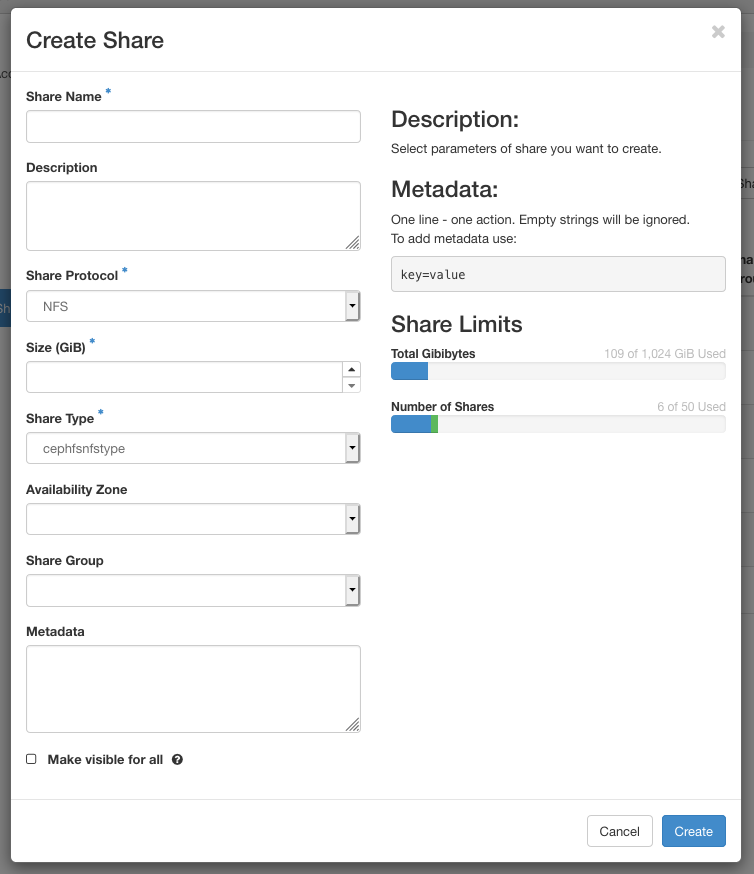
\includegraphics[width=0.7\textwidth]{img/create_share}
  \end{center}
  Fill out the following fields:
  \begin{description}
  \item[Share Name] Choose a name.
  \item[Description] Optionally, add a description.
  \item[Share Protocol] Use the default \gls{nfs} protocol.
  \item[Size (GiB)] Set the size of the shared file system to be
    created.  The total available storage and the amount currently
    used are shown on the right.
  \item[Share Type] Here, you must select ``cephfsnfstype'' (the only choice).
  \item[Metadata] You can attach additional metdata to your shared
    file system, which can be queried later on.
  \end{description}
  Other fields are not mandatory.  By default, the shared file system
  will only be visible within the current project (Visibility:
  ``private'').  Be careful with the option ``Make visible for all':
  enabling it will set the visibility of your shared file system to
  ``public'', making it visible for any other project in the VSC cloud
  as well.
\item Click \textbf{Create} to complete this step.
\end{enumerate}
% https://docs.openstack.org/security-guide/shared-file-systems/share-acl.html

At this point, the shared file system exists within OpenStack, but it cannot be used until we define access rules for it.

\section*{Defining \gls{nfs} access rules}\label{sec:defin-nfs-access}
You must define rules that define which machines on the network may
obtain read or write access to your shared file system.  By default,
in absence of any rules, a shared file system cannot be accessed by
anyone.

%TODO screenshots?
\begin{enumerate}
\item Open the drop-down menu in the \textbf{Actions} column for your share, and click \textbf{Manage Rules}.
\item You can now see all Share Rules for this shared file system.
  For a newly created file system, the list will be empty.  Click \textbf{Add rule}.
\item Fill out the \textbf{Add Rule} dialog:
  \begin{description}
  \item[Access Type] Only ``ip'' is supported.
  \item[Access Level] Choose if you want to give read and write
    (``rw'') or read-only (``ro'') permission with this rule.
  \item[Access To] Here, you can specify an ip address, or an address
    range, to which the rule applies.  The addresses should be
    specified according to the format expected by an NFS exports
    configuration file.  The following table contains a few examples,
    where it is assumed that the project's \_nfs network has the
    address range 10.10.x.0/24:

    \begin{tabular}{>{\bfseries}lp{0.7\textwidth}}
      10.10.x.13 & Allow this single ip address.
      \\ \hline
      0.0.0.0/0 & Allow any ip address.
      \\ \hline
      10.10.x.0/24 & Allow any ip address from the project's \_nfs network.  For a non-public shared file system this has the same effect as the previous rule, because such a shared file system can only be accessed from within our project's \_nfs network anyway.
      \\ \hline 
      10.10.x.0/28 & Allow addresses 10.10.x.0 until 10.10.x.15.
      \\
    \end{tabular}

  \end{description}
  Click \textbf{Add} to add the rule.
\end{enumerate}
Your rule now appears in the list.  You can add as many rules as you
wish, to set the access level for different addresses or address
ranges.

\section*{Accessing a shared file system}\label{sec:access-shar-file}
When the proper access rules for the shared file system are in place,
you can access it from an instance with a matching ip.  In order to be
able to mount the shared file system, your instance needs
\begin{itemize}
\item a \gls{nfs} client, installed by default on images provided by
  the VSC cloud, and
\item access to the \_nfs network.  Because your instance likely has to
  connect to the \_vm network as well, your VM should have two
  \gls{nic}'s.  Again, this is taken care of in the default images.
\end{itemize}

When you are ready to mount the network file system on an instance,
look up the network location of your file system using the Dashboard:
\begin{enumerate}
\item Open the Share tab and click Shares.  The list of all shared file systems in your project is shown.
\item Click the name of the shared file system you wish to access.
\item In the section ``Share Overview'', look for the item \textbf{Export locations}.
\item Copy the content of the \textbf{Path:} field.
\end{enumerate}

Once you know the location of your shared file system, you can mount
it on any VM with the appropriate access rights, e.g.\ for a shared
file system with location
\lstinline{10.2.0.2:/volumes/_nogroup/918...a78:}

\begin{prompt}
  %\shellcmd{sudo mount 10.2.0.2:/volumes/\_nogroup/918..a78 /mnt}
\end{prompt}
%%% Local Variables:
%%% mode: latex
%%% TeX-master: "intro-OpenStack"
%%% End:


\chapter{Appendix}

\section{VSC Tier-1 Cloud flavors list}\label{sec:appendix-flavors}


\begin{prompt}
$ openstack flavor list
+----+-----------------+--------+------+-----------+-------+-----------+
| ID | Name            |    RAM | Disk | Ephemeral | VCPUs | Is Public |
+----+-----------------+--------+------+-----------+-------+-----------+
| 0  | CPUv1.nano      |     64 |    1 |         0 |     1 | True      |
| 1  | CPUv1.tiny      |    512 |   10 |         0 |     1 | True      |
| 10 | UPSv1.medium    |   4096 |   30 |         0 |     2 | True      |
| 11 | UPSv1.large     |   8192 |   40 |         0 |     4 | True      |
| 12 | UPSv1.2xlarge   |  61440 |   40 |         0 |    16 | True      |
| 13 | GPUv1.small     |   2048 |   20 |         0 |     1 | True      |
| 14 | GPUv1.medium    |   4096 |   30 |         0 |     2 | True      |
| 15 | GPUv1.large     |   8192 |   40 |         0 |     4 | True      |
| 16 | GPUv1.2xlarge   |  61440 |   40 |         0 |    16 | True      |
| 17 | UPSv1.3xlarge   | 122880 |   80 |         0 |    16 | True      |
| 18 | CPUv1.1_3xlarge | 184320 |   80 |         0 |    14 | True      |
| 19 | CPUv1.4xlarge   | 368640 |   80 |         0 |    20 | True      |
| 2  | CPUv1.small     |   2048 |   20 |         0 |     1 | True      |
| 3  | CPUv1.medium    |   4096 |   30 |         0 |     2 | True      |
| 4  | CPUv1.large     |   8192 |   40 |         0 |     4 | True      |
| 5  | CPUv1.xlarge    |  16384 |   40 |         0 |     8 | True      |
| 6  | CPUv1.2xlarge   |  61440 |   40 |         0 |    16 | True      |
| 7  | CPUv1.3xlarge   | 122880 |   80 |         0 |    16 | True      |
| 8  | CPUv1.1_2xlarge |  61440 |   40 |         0 |     8 | True      |
| 9  | UPSv1.small     |   2048 |   20 |         0 |     1 | True      |
+----+-----------------+--------+------+-----------+-------+-----------+
\end{prompt}

%%% Local Variables:
%%% mode: latex
%%% TeX-master: "intro-Cloud"
%%% End:


\end{document}

%%% Local Variables:
%%% mode: latex
%%% TeX-master: t
%%% End:
